% Task C14
% Source volume: lower
% Physical scan pages: 52--90
% Printed book pages: 40--78
% Transcribe only source content; omit running headers, footers, and printed page numbers.
\chapter{函数项级数与幂级数}

% BEGIN TRANSCRIPTION

无穷级数为研究函数提供了全新的有力工具，如果说数项级数是无穷级数的基础，则函数项级数就是无穷级数的理论核心。

本章共分五节，前两节是函数项级数的一般理论。在 §14.1 中，我们讨论函数项级数与函数列的一致收敛性；§14.2 是和函数与极限函数性质的讨论。接下来的两节用于讨论最重要的一类函数项级数——幂级数。§14.3 为其一般理论，§14.4 为 Taylor 级数展开。最后一节是学习要点和两组参考题。

\section{一致收敛性及其判别法}

函数是数学分析的主要研究对象。将函数展开为函数项级数，使得级数的通项是比较简单的函数，这样就为函数的研究和计算提供了新工具。对于以函数项级数的和函数形式出现的大量非初等函数，如何利用级数来研究它们的基本性质，如连续性、可微性、可积性以及如何计算它们的导数和积分就成为需要解决的基本理论问题。为此我们需要引进新的概念，这就是一致收敛性。

\subsection{基本内容}

下面先列出函数项级数的一致收敛概念的要点。

1. 函数项级数 $\displaystyle\sum_{n=1}^{\infty}u_n(x)$ 在某个数集 $E$ 上的收敛性以及在收敛时的和函数（值）是逐点定义的，一般称为“点收敛”“逐点收敛”或“点态收敛”等。这在上一章都已见过，在讨论时与常数项级数没有区别。但为了研究函数项级数的和函数，则需要有比点收敛更强的条件，这就是一致收敛性。在 [31] 的第六章中有这方面发展的历史性材料。

2. 函数项级数在数集 $E$ 上的一致收敛性是一种整体性质。这类整体性质在数学分析中多次出现。例如函数在某个区间上的有界性、一致连续性和 Riemann 可积性等。与此相反，函数的连续性、可微性和函数项级数的点收敛性则是局部性质（可参考上册 137，140 页）。

3. 称函数项级数 $\displaystyle\sum_{n=1}^{\infty}u_n(x)$ 在数集 $E$ 上一致收敛，如果该级数的部分和函数列 $\{S_n(x)\}$ 在 $E$ 上一致收敛。

4. 设一个函数列 $\{S_n(x)\}$ 在数集 $E$ 上收敛于其极限函数 $S(x)$。称 $\{S_n(x)\}$ 于 $E$ 上一致收敛，如果对于每个正数 $\varepsilon>0$，存在 $N$，使得对每个正整数 $n>N$，和每个 $x\in E$，均成立
\[
  \abs{S_n(x)-S(x)}<\varepsilon.
\]
容易看出，这与 $\displaystyle\lim_{n\to\infty}S_n(x)=S(x)$ 在所有 $x\in E$ 成立的不同之处是目前的 $N$ 只与 $\varepsilon$ 有关，它对于所有 $x\in E$ 同时适用，这就是收敛的“一致性”。

5. 若函数项级数 $\displaystyle\sum_{n=1}^{\infty}u_n(x)$ 在开区间 $I$ 中的每个有界闭区间上一致收敛，则称该级数在 $I$ 中\textbf{内闭一致收敛}。与函数的有界性、一致连续性和可积性等整体性质一样，若一个函数项级数在 $I$ 上一致收敛，则一定在 $I$ 中内闭一致收敛，但反之不一定成立。

6. 若 $\displaystyle\sum_{n=1}^{\infty}\abs{u_n(x)}$ 于数集 $E$ 上一致收敛，则称 $\displaystyle\sum_{n=1}^{\infty}u_n(x)$ 于 $E$ 上\textbf{绝对一致收敛}。在 $E$ 上绝对一致收敛的函数项级数必在 $E$ 上一致收敛，但反之不真。

一致收敛性有明显的几何意义。下面是三个例子及其几何图像。

\begin{xexample}[14.1.1]
非负连续函数列 (1) $\{x\ee^{-nx}\}$，(2) $\{nx\ee^{-nx}\}$，(3) $\{n^2x\ee^{-nx}\}$ 在区间 $[0,1]$ 上收敛于同一个极限函数 $S(x)=0$。从图 14.1 上可以看出它们在 $[0,1]$ 上的收敛情况大不相同。(1) 是一致收敛的；(2) 不一致收敛，但还是一致有界的；(3) 不一致收敛，而且不一致有界。（图中对 (3) 只作出 $0\leqslant x\leqslant0.1$ 的部分。）
\end{xexample}

\begin{center}
  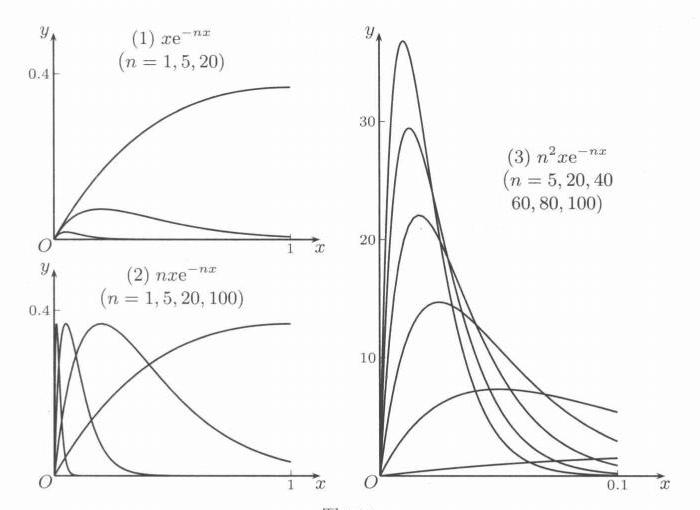
\includegraphics[width=.78\linewidth]{figures/lower/ch14/fig-14-1.png}

  图 14.1
\end{center}

容易看出三个函数列中的第 $n$ 个函数都在点 $x=1/n$ 处达到最大值。这些最大值分别为 $1/(n\ee),1/\ee$ 和 $n/\ee$。又不难计算出，对这三个函数列都存在（曲边梯形面积的）极限 $\displaystyle\lim_{n\to\infty}\int_0^1 f_n(x)\,\dd x$，极限值分别为 $0,0$ 和 $1$。

其次是一致收敛性的判别方法。

1. 对于函数项级数来说，主要的一致收敛性判别法有：Cauchy 一致收敛准则、Weierstrass 判别法（也称为 M-判别法、强级数判别法和优级数判别法等），以及通过 Abel 变换得到的 Abel 判别法和 Dirichlet 判别法。

2. Cauchy 一致收敛准则是充分必要条件，但应用时往往需要较复杂的技巧。

3. Weierstrass 判别法只对绝对一致收敛的情况有效，但是可举例说明，存在绝对一致收敛的函数项级数的例子，使得 Weierstrass 判别法失效。但由于它将问题归结为正项级数的收敛性判别，使用方便，因此有广泛的应用。

4. Abel 判别法和 Dirichlet 判别法都是函数项级数一致收敛的充分必要条件，其证明与广义积分和数项级数的同名判别法类似。

5. 在数项级数中没有对应物的是基于 Dini 定理的 Dini 判别法：

\begin{xtheorem}[Dini 定理]
若函数项级数 $\displaystyle\sum_{n=1}^{\infty}u_n(x)$ 的每一项（或 $n$ 充分大后的项）为有界闭区间 $[a,b]$ 上的非负连续函数，又已知级数的和函数 $S(x)$ 也在 $[a,b]$ 上连续，则级数在 $[a,b]$ 上一致收敛。\footnote{Dini 定理对于非有界闭区间不成立，例如对于函数列来说，在 $[0,1)$ 上的函数列 $\{x^n\}$ 处处单调收敛于 $0$，但不一致收敛。}
\end{xtheorem}

当然 Dini 判别法对条件的要求较高，但它仍在许多问题中有效。此外，如果关心的区间不是有界闭区间，则还有可能得到内闭一致收敛性的结论。

6. 在讨论函数项级数 $\displaystyle\sum_{n=1}^{\infty}u_n(x)$ 的一致收敛性时比较容易的一类情况是能够得到其部分和函数列 $\{S_n(x)\}$ 的紧凑表达式，这时问题就转化为\textbf{函数列的一致收敛性问题}（不难看出可以将已经列举的各种判别法改述为关于函数列的一致收敛性判别法）。如果同时还能得到级数的和函数，即函数列 $\{S_n(x)\}$ 的极限函数 $S(x)$ 的表达式，则就有\textbf{上确界判别法}：函数列 $\{S_n(x)\}$ 在数集 $E$ 上一致收敛于 $S(x)$ 的充分必要条件是
\[
  \lim_{n\to\infty}\sup_{x\in E}\{\abs{S_n(x)-S(x)}\}=0.
\]
对于具体问题来说，则往往有可能用微分法求 $\abs{S_n(x)-S(x)}$ 在 $E$ 上的最大值或上确界，又若能估计出它的上界 $a_n$ 使得成立 $\displaystyle\lim_{n\to\infty}a_n=0$，则也可以得到一致收敛的结论。这也可称为\textbf{优势判别法}。

这里需要指出几点：

(1) 请初学者注意：这个上确界判别法（即优势判别法）与函数项级数的 Weierstrass 判别法不一样，并无直接关系，前者是充分必要条件，后者只是充分条件。

(2) 由于上确界判别法是充分必要条件，因此往往能解决不一致收敛的判别问题。特别是还能得到以下的\textbf{对角线判别法}：如果存在数列 $\{x_n\}\subset E$，使得条件
\[
  \lim_{n\to\infty}\abs{S_n(x_n)-S(x_n)}=0
\]
不满足，则 $\{S_n(x)\}$ 在 $E$ 上不一致收敛于 $S(x)$。

(3) 为了便于掌握有关一致收敛的基本概念，在教科书中均举出许多可以用上确界判别法得到解决的例题。但是这并不表明这类方法可以用于许多函数项级数问题上去。事实上求函数项级数的部分和函数列以及和函数的表达式一般是困难的或者根本做不到的事情。

7. 证明给定的函数项级数在某个数集 $E$ 上不一致收敛的方法不多。如果不能将问题归结为函数列去研究的话，则一般需要用 Cauchy 一致收敛准则。此外，在一致收敛条件下保证和函数或极限函数具有某种性质的一系列命题的逆否命题，也往往可以用来判定非一致收敛性。最常用的就是连续性命题的逆否命题：若函数项级数（或函数列）的每一项于区间 $I$ 上处处连续，又已知其和函数（或极限函数）在 $I$ 上不是处处连续，则级数（或函数列）于 $I$ 上不一致收敛。在下面例题 14.1.3 中还会介绍它的一种变形。

\subsection{例题}

由于在一般教科书中已有大量关于函数列的例题，本节不拟收入这方面的很多材料。下面首先是几个涉及判别方法的例题。

\begin{xexample}[14.1.2]
绝对一致收敛的函数项级数的一致收敛性不一定能够用 Weierstrass 判别法来判定：观察非负函数项级数 $\displaystyle\sum_{n=1}^{\infty}u_n(x)$，其中对 $n=1,2,\ldots$，令
\[
  u_n(x)=
  \begin{cases}
    \dfrac1n,& \dfrac1{n+1}\leqslant x<\dfrac1n,\\[4pt]
    0,& x\in[0,1]\text{ 的其他情形}.
  \end{cases}
\]
容易看出，对于区间 $[0,1]$ 中的每个 $x$，在级数的无限项中至多只有一项不是 $0$，因此级数处处收敛，又可以看出对余项的估计
\[
  R_n(x)=\sum_{k=n+1}^{\infty}u_k(x)\leqslant\frac1{n+1}
\]
在 $[0,1]$ 上一致成立，因此级数在 $[0,1]$ 上一致收敛。但是从 $\displaystyle\sup_{x\in[0,1]}\{u_n(x)\}=\frac1n$（$n=1,2,\ldots$）和调和级数发散可知，用 Weierstrass 判别法一定不成功。
\end{xexample}

\begin{xremark}
本题的构造方法可以推广为：设非负数列 $\{a_n\}$ 收敛于 $0$，区间 $I$ 上的函数列 $\{u_n(x)\}$ 满足条件 $\abs{u_n(x)}\leqslant a_n,\ \forall n$，$u_i(x)u_j(x)=0,\ \forall i\ne j$，则 $\displaystyle\sum_{n=1}^{\infty}u_n(x)$ 在区间 $I$ 上必一致收敛。
\end{xremark}

下一个例题中的结论可以作为一种\textbf{不一致收敛判别法}来使用。

\begin{xexample}[14.1.3]
设对每个 $n$，函数 $u_n(x)$ 在 $x=c$ 处左连续，又已知 $\displaystyle\sum_{n=1}^{\infty}u_n(c)$ 发散。证明：对任意正数 $\delta>0$，$\displaystyle\sum_{n=1}^{\infty}u_n(x)$ 在区间 $(c-\delta,c)$ 上必不一致收敛。
\end{xexample}
\begin{xproof}
用反证法。设有 $\delta>0$，使 $\displaystyle\sum_{n=1}^{\infty}u_n(x)$ 在区间 $(c-\delta,c)$ 上一致收敛，这就是
\[
  \forall\varepsilon>0,\ \exists N>0,\ \text{当 }n\geqslant N\text{ 时，对每个正整数 }p\text{ 和每个 }x\in(c-\delta,c),\text{ 成立}
\]
\begin{equation}
  \abs{u_{n+1}(x)+u_{n+2}(x)+\cdots+u_{n+p}(x)}<\varepsilon.
  \tag{14.1}
  \label{eq:14.1}
\end{equation}
由题设，$u_{n+1}(x)+u_{n+2}(x)+\cdots+u_{n+p}(x)$ 在 $x=c$ 左连续，在 (14.1) 中令 $x\to c^-$，得到
\[
  \abs{u_{n+1}(c)+u_{n+2}(c)+\cdots+u_{n+p}(c)}\leqslant\varepsilon.
\]
由数项级数的 Cauchy 收敛准则知道，这与 $\displaystyle\sum_{n=1}^{\infty}u_n(c)$ 发散的条件相矛盾。
\end{xproof}

\begin{xremark}
可将本题与一致连续性理论中的例题 5.4.5（上册 140 页）作比较。
\end{xremark}

\begin{xremark}
例如，函数项级数 $\displaystyle\sum_{n=1}^{\infty}n\ee^{-nx}$ 在 $x=0$ 时发散，因此该级数在 $(0,+\infty)$ 上必定不一致收敛。当然，还可以进一步研究是否内闭一致收敛等可能性。
\end{xremark}

下一个例题是用导函数的性质来判定函数项级数的一致收敛性。

\begin{xexample}[14.1.4]
\textbf{（Bendixon（本迪克松）判别法）} 设 $\displaystyle\sum_{n=1}^{\infty}u_n(x)$ 为 $[a,b]$ 上的可微函数项级数，且 $\displaystyle\sum_{n=1}^{\infty}u_n'(x)$ 的部分和函数列在 $[a,b]$ 上一致有界，证明：如果 $\displaystyle\sum_{n=1}^{\infty}u_n(x)$ 在 $[a,b]$ 上收敛，则必在 $[a,b]$ 上一致收敛。
\end{xexample}
\begin{xproof}
由题设，存在正常数 $C$，使得对每个正整数 $n$ 和每个 $x\in[a,b]$，同时成立不等式
\[
  \abs{\sum_{k=1}^{n}u_k'(x)}\leqslant C.
\]
对每个给定的 $\varepsilon>0$，取区间 $[a,b]$ 的等距分划 $\{x_0,x_1,\ldots,x_m\}$，其中 $m$ 充分大，使分划的细度
\[
  \Delta x_i=\frac{b-a}{m}<\frac{\varepsilon}{4C}.
\]
由于函数项级数 $\displaystyle\sum_{n=1}^{\infty}u_n(x)$ 在 $[a,b]$ 上处处收敛，因此从 Cauchy 收敛准则知，存在 $N$，使 $n>N$ 时，对任意正整数 $p$ 和分划的每个分点 $x_i$，同时成立
\[
  \abs{\sum_{k=n+1}^{n+p}u_k(x_i)}<\frac{\varepsilon}{2},\qquad i=0,1,\ldots,m.
\]
现在对于任意的 $x\in[a,b]$，不妨设 $x\in[x_{i-1},x_i]$，就可以作出估计：
\[
\begin{aligned}
  \abs{\sum_{k=n+1}^{n+p}u_k(x)}
  &=\abs{\sum_{k=n+1}^{n+p}u_k(x_i)+\sum_{k=n+1}^{n+p}(u_k(x)-u_k(x_i))}\\
  &\leqslant \abs{\sum_{k=n+1}^{n+p}u_k(x_i)}+\abs{\sum_{k=n+1}^{n+p}u_k'(\xi_i)}\,\abs{x-x_i}\\
  &<\frac{\varepsilon}{2}+2C\abs{x-x_i}\leqslant\frac{\varepsilon}{2}+\frac{\varepsilon}{2}=\varepsilon,
\end{aligned}
\]
其中在 $[x,x_i]$ 上对 $\displaystyle\sum_{k=n+1}^{n+p}[u_k(x)-u_k(x_i)]$ 用微分中值定理，$\xi_i\in(x,x_i)$。这表明 $\displaystyle\sum_{n=1}^{\infty}u_n(x)$ 在 $[a,b]$ 上满足 Cauchy 一致收敛准则，从而在 $[a,b]$ 上一致收敛。
\end{xproof}

\begin{xexample}[14.1.5]
证明：函数项级数 $\displaystyle\sum_{n=1}^{\infty}(-1)^n x^n(1-x)$ 在 $[0,1]$ 上绝对收敛且一致收敛，但不绝对一致收敛。
\end{xexample}
\begin{xproof}
(1) $\displaystyle\sum_{n=1}^{\infty}(-1)^n x^n(1-x)$ 在 $[0,1]$ 上绝对收敛：实际上每项取绝对值之后的级数 $\displaystyle\sum_{n=1}^{\infty}x^n(1-x)$ 的部分和函数列为 $\{x-x^{n+1}\}$，因此在 $[0,1]$ 上处处收敛。

(2) $\displaystyle\sum_{n=1}^{\infty}(-1)^n x^n(1-x)$ 在 $[0,1]$ 上不绝对一致收敛：从 (1) 可见取绝对值后级数 $\displaystyle\sum_{n=1}^{\infty}x^n(1-x)$ 的和函数为 $S(x)=x,\ x\in[0,1)$，$S(1)=0$，它在点 $x=1$ 的左侧不连续，而级数通项在 $[0,1]$ 上连续，因此该级数在 $[0,1]$ 上不一致收敛。

(3) $\displaystyle\sum_{n=1}^{\infty}(-1)^n x^n(1-x)$ 在 $[0,1]$ 上一致收敛：直接计算出余项
\[
  R_n(x)=\sum_{k=n+1}^{\infty}(-1)^k x^k(1-x)=\frac{(-1)^{n+1}x^{n+1}(1-x)}{1+x},
\]
因此有估计（其中利用了算术平均值--几何平均值不等式）：
\[
\begin{aligned}
  \abs{R_n(x)}&\leqslant(1-x)x^{n+1}
  =\frac1{n+1}[(n+1)(1-x)\cdot x^{n+1}]\\
  &\leqslant\frac1{n+1}\left(\frac{n+1}{n+2}\right)^{n+2}
  <\frac1{n+1}\to0,
\end{aligned}
\]
可见级数于 $[0,1]$ 上一致收敛。
\end{xproof}

\begin{xexample}[14.1.6]
求 $\displaystyle\sum_{n=1}^{\infty}n\left(x+\frac1n\right)^n$ 的收敛域，并讨论其一致收敛性。
\end{xexample}
\begin{xsolution}
(1) 先求收敛域。当 $x=0$ 时级数显然收敛。当 $x\ne0$ 时，观察级数通项的绝对值：
\[
  \abs{n\left(x+\frac1n\right)^n}
  =n\abs{x}^n\cdot\abs{1+\frac1{nx}}^n\sim n\abs{x}^n\ee^{1/x},
\]
因而原级数当 $\abs{x}<1$ 时收敛，当 $\abs{x}\geqslant1$ 时发散，级数的收敛域是 $(-1,1)$。

(2) 函数项级数一致收敛的一个必要条件是其通项一致收敛于 $0$，但本题的级数通项不满足这个条件。这用对角线判别法就可以知道：对每个正整数 $n$，取 $x_n=1-\dfrac1n\in(-1,1)$，则就有
\[
  n\left(x_n+\frac1n\right)^n=n\to+\infty.
\]
因此所论级数在 $(-1,1)$ 上不一致收敛。
\end{xsolution}

\begin{xremark}
这里也可用例题 14.1.3 提供的判别法。由于当 $\abs{x}=1$ 时级数发散，因此不可能在 $(-1,1)$ 上一致收敛。但是容易证明级数在其中内闭一致收敛。
\end{xremark}

下一题在每种教科书中都有，为了比较起见，我们列入该题，证明从略。

\begin{xexample}[14.1.7]
证明：级数 $\displaystyle\sum_{n=1}^{\infty}\frac{\sin nx}{n}$ 在闭区间 $[a,b]$ 上一致收敛的充分必要条件是该闭区间不含 $2\pi$ 的整数倍点。
\end{xexample}

下面是用 Cauchy 一致收敛准则来判定函数项级数的经典性结果，其中所用的分析方法具有新的特点，值得学习（参见 [51]）。

\begin{xexample}[14.1.8]
设 $\{b_n\}$ 为单调减少的非负数列，证明：级数 $\displaystyle\sum_{n=1}^{\infty}b_n\sin nx$ 在 $(-\infty,+\infty)$ 上一致收敛的充分必要条件是 $b_n=\littleo\left(\dfrac1n\right)$。
\end{xexample}
\begin{xproof}
为方便起见引入下列记号，其中 $n<p$：
\[
  S_{n,p}=b_n\sin nx+b_{n+1}\sin(n+1)x+\cdots+b_p\sin px.
\]
先证必要性。此时只需考虑区间 $(0,1)$。设级数在这个区间上一致收敛，则对于 $\varepsilon>0$，存在 $N$，使得对于任意的 $p>n>N$，不等式 $\abs{S_{n,p}}<\varepsilon$ 对所有 $x\in(0,1)$ 同时成立。

取 $p=2n-1$，$x=\dfrac{\pi}{4n}$，这时在和式
\[
  S_{n,2n-1}=b_n\sin nx+b_{n+1}\sin(n+1)x+\cdots+b_{2n-1}\sin(2n-1)x
\]
中的每个正弦函数的自变量都在区间 $\left[\dfrac\pi4,\dfrac\pi2\right]$ 中，因此就有
\[
  b_{2n}n\sin\frac\pi4<b_{2n}[\sin nx+\sin(n+1)x+\cdots+\sin(2n-1)x]\leqslant S_{n,2n-1}<\varepsilon,
\]
可见 $b_n=\littleo\left(\dfrac1n\right)$ 成立。

再证充分性。显然只要证明级数在区间 $[0,\pi]$ 上一致收敛。这时对 $S_{n,p}$ 的估计将随 $x$ 取不同值而采用不同的方法，但最后综合起来的估计则与 $x$ 无关。

从非负无穷小量 $\{nb_n\}$ 可以合理地定义一个新的单调减少数列：
\[
  \mu_n=\max_{m\geqslant n}\{mb_m\},\qquad n=1,2,\ldots,
\]
且有 $\mu_n\to0$。以下分三种情况估计 $S_{n,p}$。

(1) 若 $x\leqslant\dfrac\pi p$，则在 $S_{n,p}$ 中的每一个正弦函数的自变量都在 $[0,\pi]$ 内，再利用 $\sin\theta\leqslant\theta,\ \forall\theta\in[0,\pi]$，就得到
\[
  \abs{S_{n,p}}=S_{n,p}\leqslant b_nnx+b_{n+1}(n+1)x+\cdots+b_ppx\leqslant p\mu_nx\leqslant\pi\mu_n.
\]

(2) 若 $x\geqslant\dfrac\pi n$，则利用三角变换（见例题 13.3.3）、Jordan 不等式 $\sin\theta\geqslant\dfrac2\pi\theta,\ \forall\theta\in[0,\dfrac\pi2]$（例题 8.5.6）和 $\dfrac x2\leqslant\dfrac\pi2$，可以对于任意 $r\geqslant n$ 估计出
\[
  \abs{\sin nx+\sin(n+1)x+\cdots+\sin rx}\leqslant\frac1{\sin(x/2)}\leqslant\frac\pi x\leqslant n,
\]
然后从 Abel 变换和 $\{b_n\}$ 的非负单调性（见 (13.22)）得到
\[
  \abs{S_{n,p}}\leqslant\frac\pi x\,b_n<nb_n\leqslant\mu_n.
\]

(3) 若 $\dfrac\pi p<x<\dfrac\pi n$，则需同时使用以上两种方法。分析 $S_{n,p}=S_{n,k}+S_{k+1,p}$，其中取 $k=[\pi/x]$（使得 $n\leqslant k<p$），并分别用前面的两种方法估计，就得到
\[
  \abs{S_{n,p}}\leqslant\abs{S_{n,k}}+\abs{S_{k+1,p}}\leqslant\pi\mu_n+\mu_{k+1}\leqslant\mu_n(\pi+1),
\]
其中利用了 $kx\leqslant\pi<(k+1)x$ 和 $\mu_{k+1}\leqslant\mu_n$。

合并 (1)--(3)，就得到估计式 $\abs{S_{n,p}}\leqslant\mu_n(\pi+1)$ 对于任意 $p>n$ 和 $x\in[0,\pi]$ 同时成立。由于 $\mu_n\to0$，可见级数一致收敛。
\end{xproof}

\begin{xremark}
例题 14.1.7 中的级数显然不满足本题的条件。
\end{xremark}

\begin{xremark}
用本题的方法（或其他方法）可以证明例题 14.1.7 中级数的部分和函数列在 $(-\infty,+\infty)$ 上一致有界。用 Dirichlet 判别法就得到比本题较弱的结论：若 $\{nb_n\}$ 单调减少趋于 $0$，则函数项级数 $\displaystyle\sum_{n=1}^{\infty}b_n\sin nx$ 在 $(-\infty,+\infty)$ 上一致收敛。
\end{xremark}

下一个例题为 §16.3 中的 Weierstrass 逼近定理的证明提供了一个初等起点，同时又可以看成是 §2.6 中迭代生成数列方法在函数列中的延伸。

\begin{xexample}[14.1.9]
\textbf{（Visser（维塞）定理）} 设在区间 $[-1,1]$ 上定义函数列 $\{a_n(x)\}$ 如下：
\[
  a_1(x)=0,\qquad a_{n+1}(x)=a_n(x)+\frac12[x^2-a_n^2(x)],\qquad n=1,2,\ldots.
\]
证明：$\{a_n(x)\}$ 是在区间 $[-1,1]$ 上一致收敛于 $\abs{x}$ 的多项式序列。
\end{xexample}

\textbf{分析}\quad 从对称性可见只需在区间 $[0,1]$ 上讨论。不难知道本题中由迭代得到的多项式序列 $\{a_n(x)\}$ 是在 $[0,1]$ 上的严格单调增加的连续函数列，且收敛于极限函数 $a(x)=x$。因此用 Dini 定理就知道结论成立。其中的具体细节请读者完成。

这里将从 §2.6 的迭代生成数列的几何理论出发，配合图 14.2 观察本题，说明如何在分析论证之前就可以发现以上全部事实。

\begin{center}
  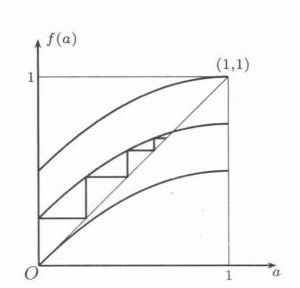
\includegraphics[width=.38\linewidth]{figures/lower/ch14/fig-14-2.png}

  图 14.2
\end{center}

考虑 $[0,1]$ 上的点收敛，则从 $a_n$ 到 $a_{n+1}$ 的迭代方程是
\begin{equation}
  f(a)=a+\frac12(x^2-a^2),
  \tag{14.2}
  \label{eq:14.2}
\end{equation}
其中 $x$ 是参数，初始值 $a_1=0$。如图 14.2 所示，其中作出了迭代方程的三条曲线，它们的参数分别为 $x=0,\dfrac{\sqrt2}{2},1$。在图中还对于中间一条曲线用 2.6.2 小节中的\textbf{蛛网工作法}从 $a_1=0$ 开始作了几次迭代（参见上册 50 页的图 2.4）。容易看到，由于参数 $x\in[0,1]$ 时的每条迭代曲线都严格单调增加，因此所得到的迭代生成数列 $\{a_n(x)\}$ 也严格单调增加。此外，对每个参数 $x\in[0,1]$ 都有
\[
  \lim_{n\to\infty}a_n(x)=x,
\]
即收敛于迭代方程 (14.2) 的不动点 $a=x$。这些都可以从关于迭代数列的两个基本规律的命题 2.6.1 和 2.6.2 直接得出。

\subsection{练习题}

\begin{xexercise}
\begin{enumerate}
  \item 讨论函数列或函数项级数在给定区间上的一致收敛性：
  \begin{enumerate}[label=(\arabic*)]
    \item $S_n(x)=\dfrac{x}{1+n^2x^2},\ n=1,2,\ldots,\ x\in(-\infty,+\infty)$；
    \item $S_n(x)=\dfrac{nx}{1+n^2x^2},\ n=1,2,\ldots,\ x\in(-\infty,+\infty)$；
    \item $S_n(x)=\dfrac{n+x^2}{nx},\ n=1,2,\ldots,\ x\in(0,+\infty)$；
    \item $S_n(x)=\dfrac{x}{n}\ln\dfrac{x}{n},\ n=1,2,\ldots$；(i) $x\in(0,1)$，(ii) $x\in(0,+\infty)$；
    \item $S_n(x)=n\sin\dfrac{x}{n},\ n=1,2,\ldots$；(i) $x\in[0,a]$，(ii) $x\in(0,+\infty)$；
    \item $S_n(x)=\dfrac1n\ln(1+\ee^{-nx}),\ n=1,2,\ldots$；(i) $x\geqslant0$，(ii) $x<0$；
    \item $\displaystyle\sum_{n=1}^{\infty}\frac{n^8}{\sqrt{n!}}(x^n+x^{-n}),\quad \frac1t\leqslant\abs{x}\leqslant t,\ t>1$；
    \item $\displaystyle\sum_{n=1}^{\infty}\frac{\sin x\sin nx}{\sqrt{n+x}},\quad x>0$；
    \item $\displaystyle\sum_{n=1}^{\infty}\frac1n\left[\ee^x-\left(1+\frac{x}{n}\right)^n\right]$；(i) 有限闭区间 $[0,b]$，(ii) $[0,+\infty)$。
  \end{enumerate}
  \item 确定函数项级数 $\displaystyle\sum_{n=1}^{\infty}\frac{x^n}{1+x^{2n}}$ 的收敛域与一致收敛域。
  \item 证明：函数项级数 $\displaystyle\sum_{n=1}^{\infty}\frac{(-1)^{n-1}x^2}{(1+x^2)^n}$ 在 $(-\infty,+\infty)$ 上绝对收敛且一致收敛，但不绝对一致收敛。
  \item 证明：函数项级数 $\displaystyle\sum_{n=2}^{\infty}\ln\left(1+\frac{x}{n\ln^2n}\right)$ 在区间 $(-a,a)$ 上一致收敛，其中 $a$ 是小于 $2\ln^2 2$ 的任意固定正数。
  \item 证明：函数项级数 $\displaystyle\sum_{n=1}^{\infty}2^n\sin\frac{1}{3^nx}$ 在 $(0,+\infty)$ 上处处收敛，但不一致收敛。
  \item 证明：函数项级数 $\displaystyle\sum_{n=0}^{\infty}\int_0^x t^n\sin\pi t\,\dd t$ 在 $[0,1]$ 上一致收敛。
  \item 设 $\{f_n\}$ 是有界闭区间 $[a,b]$ 上的连续函数列，且设该函数列在 $(a,b)$ 上一致收敛，证明：$\{f_n\}$ 在点 $a$ 和 $b$ 都收敛，且在 $[a,b]$ 上一致收敛。
  \item 设 $f$ 在 $(a,b)$ 上有连续导函数，定义
  \[
    F_n(x)=\frac n2\left[f\left(x+\frac1n\right)-f\left(x-\frac1n\right)\right],\quad x\in(a,b),\ n=1,2,\ldots.
  \]
  证明：函数列 $\{F_n\}$ 在 $(a,b)$ 上处处收敛且内闭一致收敛。
  \item 设函数列 $\{u_n(x)\}$ 中的函数在 $[a,b]$ 上同为单调增加函数或同为单调减少函数，如果 $\displaystyle\sum_{n=1}^{\infty}u_n(a)$ 与 $\displaystyle\sum_{n=1}^{\infty}u_n(b)$ 都绝对收敛，证明：函数项级数 $\displaystyle\sum_{n=1}^{\infty}u_n(x)$ 在 $[a,b]$ 上一致收敛。
  \item 设在区间 $[a,b]$ 上的连续函数列 $\{f_n\}$ 一致收敛于极限函数 $f$，且已知 $f$ 在 $[a,b]$ 上无零点，证明：函数列 $\left\{\dfrac1{f_n}\right\}$ 在 $[a,b]$ 上一致收敛。
  \item 设函数列 $\{f_n\}$ 于区间 $I$ 上一致收敛，又设每个 $f_n$ 于 $I$ 上有界，证明：函数列 $\{f_n\}$ 于 $I$ 上一致有界。
  \item 设函数列 $\{f_n\}$ 与 $\{g_n\}$ 分别在区间 $I$ 上一致收敛。如果每个 $f_n$ 和 $g_n$ 在 $I$ 上有界，证明：函数列 $\{f_n\cdot g_n\}$ 在 $I$ 上一致收敛。\footnote{如允许 $f_n$（或 $g_n$）无界，则结论可不成立（见 [62] 的第二册 282 页）。}
  \item 设 $f\in C(-\infty,+\infty)$，定义函数列
  \[
    S_n(x)=\sum_{k=1}^{n}\frac1n f\left(x+\frac{k}{n}\right),\quad n=1,2,\ldots,
  \]
  证明：函数列 $\{S_n(x)\}$ 在 $(-\infty,+\infty)$ 上内闭一致收敛。
  \item 设 $S_1(x)\in R[a,b]$，定义
  \[
    S_{n+1}(x)=\int_a^x S_n(t)\,\dd t,\quad n=1,2,\ldots.
  \]
  证明：函数列 $\{S_n(x)\}$ 在 $[a,b]$ 上一致收敛。
\end{enumerate}
\end{xexercise}

\section{和函数与极限函数的性质}

\subsection{三分法与极限顺序交换原理}

这里的基本问题是从函数项级数 $\displaystyle\sum_{n=1}^{\infty}u_n(x)$ 中的 $\{u_n(x)\}$（或函数列 $\{S_n(x)\}$）出发去研究级数的和函数（或函数列的极限函数）的性质以及进行各种分析运算。

由于所关心的性质和运算本身都涉及极限运算，因此就必然遇到\textbf{两个（或两个以上）极限过程的顺序交换问题}。实际上在上册 10.2.3 小节的对积分求极限中已经遇到这类问题，但那时还不能进行一般性讨论。

在学习函数项级数的基础上，就可以比较系统地研究极限顺序交换问题。大致来说，对于本节所提出的问题，最基本的概念就是一致收敛性。有关的基本结论在教科书中均已有详细叙述，这里不必重复。本节主要是指出其中的一些重要问题，以作为教科书的补充。

从极限顺序交换角度出发，下列命题看似平淡，实际上具有很基本的意义，我们将从方法的角度来分析它的证明，而不是简单地重复教科书中的证明。

\begin{xproposition}[14.2.1]
设函数列 $\{S_n(x)\}$ 在点 $x_0$ 的某个邻域 $U(x_0)$ 上一致收敛于函数 $S(x)$，且对每个正整数 $n$，极限 $\displaystyle\lim_{x\to x_0}S_n(x)$ 存在且有限，则 $\displaystyle\lim_{n\to\infty}\lim_{x\to x_0}S_n(x)$ 与 $\displaystyle\lim_{x\to x_0}S(x)$ 都存在且两者相等，这就是
\begin{equation}
  \lim_{n\to\infty}\lim_{x\to x_0}S_n(x)=\lim_{x\to x_0}\lim_{n\to\infty}S_n(x).
  \tag{14.3}
  \label{eq:14.3}
\end{equation}
\end{xproposition}

\textbf{分析与证明}\quad 引入记号 $\displaystyle\lim_{x\to x_0}S_n(x)=a_n,\ n=1,2,\ldots$。

(1) 先证明 (14.3) 左边的 $\displaystyle\lim_{n\to\infty}a_n$ 收敛。因为 $\{S_n(x)\}$ 在 $x_0$ 的邻域 $U(x_0)$ 上一致收敛于函数 $S(x)$，所以由 Cauchy 一致收敛准则知，对每个给定的 $\varepsilon>0$，存在 $N$，使得对于任意的 $n,m>N$ 和所有的 $x\in U(x_0)$，同时成立
\[
  \abs{S_n(x)-S_m(x)}<\varepsilon.
\]
在此不等式中令 $x\to x_0$ 就有
\[
  \abs{a_n-a_m}\leqslant\varepsilon.
\]
这表明数列 $\{a_n\}$ 满足 Cauchy 收敛准则，因此极限 $\displaystyle\lim_{n\to\infty}a_n$ 存在。

(2) 记 $\displaystyle\lim_{n\to\infty}a_n=\lim_{n\to\infty}\lim_{x\to x_0}S_n(x)=A$。下面证明 (14.3) 右边的 $\displaystyle\lim_{x\to x_0}S(x)=A$。然而如何去估计 $\abs{S(x)-A}$？从条件可见我们无法直接估计它，而必须采取间接的（或者说曲折的）方法进行估计。这就是在分析中常用的\textbf{三分法}（也称为 $\varepsilon/3$ 法或 $3\varepsilon$ 法），即为了估计 $\abs{S(x)-A}$ 而作以下插项和分拆：
\begin{equation}
\begin{aligned}
  \abs{S(x)-A}
  &=\abs{S(x)-S_n(x)+S_n(x)-a_n+a_n-A}\\
  &\leqslant\abs{S(x)-S_n(x)}+\abs{S_n(x)-a_n}+\abs{a_n-A}.
\end{aligned}
\tag{14.4}
\label{eq:14.4}
\end{equation}
我们的目的是要证明：对于每个给定的 $\varepsilon>0$，存在 $\delta>0$，使得当 $0<\abs{x-x_0}<\delta$ 时上式左边小于 $\varepsilon$，而 (14.4) 使我们只需分别估计右边的三项。

右边第一项由于 $\{S_n(x)\}$ 在邻域 $U(x_0)$ 上一致收敛，因此只要 $n$ 足够大，就可以对该邻域中的所有 $x$ 满足该项小于 $\varepsilon/3$ 的要求。

对于 (14.4) 右边的第二项则似乎只要利用 $\displaystyle\lim_{x\to x_0}S_n(x)=a_n$：当 $x$ 与 $x_0$ 充分接近时，这一项就可小于 $\varepsilon/3$。但这里的 $n$ 取什么？是否存在 $\delta>0$，使得
\begin{equation}
  0<\abs{x-x_0}<\delta\Longrightarrow\abs{S_n(x)-a_n}<\frac\varepsilon3
  \tag{14.5}
  \label{eq:14.5}
\end{equation}
对于一切 $n$ 成立？在题设中显然没有这样的一致性条件（但是参看下面的命题 14.2.2）。

再观察 (14.4) 的第三项，由于 $a_n\to A$，因此对于 $\varepsilon$，存在 $N$，当 $n>N$ 时，就有 $\abs{a_n-A}<\varepsilon/3$ 成立。

如何将以上的分析综合起来以写出一个正确的证明？对于 (14.4) 中的第一项和第三项，可以分别取出 $N_1$ 和 $N_2$，使得当 $n>N_1$ 和 $n>N_2$ 时它们分别小于 $\varepsilon/3$。由于这两步是独立的，从而只要取 $N=\max\{N_1,N_2\}$，就可以使得当 $n>N$ 时对这两项的估计都满足要求。

最后，取定一个 $n$\footnote{这是证明的关键所在。在 (14.4) 中的插项与分拆是分析中的常用方法，根据需要也可能拆成二项或四项等。这里的困难完全在于怎样处理 (14.4) 右边的 $n$，它在左边并不出现。}，例如令 $n=N+1$，然后如前面所分析的那样，存在 $\delta>0$，使得 (14.5) 成立。这样就使得当 $\abs{x-x_0}<\delta$ 时 (14.4) 的左边小于 $\varepsilon$。

\begin{xremark}
对于命题 14.2.1 的以上分析可以使我们接触到极限顺序交换的基本原理。这里不准备详细写出这个原理，而是只讲一个大意，然后举出与命题 14.2.1 对偶的但不很常见的结论。
\end{xremark}

这个原理就是：设有在集合 $X\times Y$ 上定义的二元函数 $f(x,y)$，同时存在 $x_0\in X$ 和 $y_0\in Y$，使得对于每个 $x\in X$ 存在极限 $\displaystyle\lim_{y\to y_0}f(x,y)$，又对于每个 $y\in Y$ 存在极限 $\displaystyle\lim_{x\to x_0}f(x,y)$，并且这两个极限过程之一对于另一个变量具有一致性，则就保证以下两边的二次极限存在且相等：
\[
  \lim_{x\to x_0}\lim_{y\to y_0}f(x,y)=\lim_{y\to y_0}\lim_{x\to x_0}f(x,y).
\]
注意：这里的二元函数以及所涉及的极限过程可以很广泛，因此我们将它称为\textbf{极限顺序交换的基本原理}。命题 14.2.1 只是它的一个特例。这个原理的证明见后面 18.1.5 小节的命题 18.1.2。下面举出使得 (14.3) 成立的对偶命题。

\begin{xproposition}[14.2.2]
设函数列 $\{S_n(x)\}$ 在点 $x_0$ 的某个邻域 $U(x_0)$ 上收敛于函数 $S(x)$，又设对每个正整数 $n$，极限 $\displaystyle\lim_{x\to x_0}S_n(x)$ 存在且有限，而且这个极限过程对 $n$ 一致，则 $\displaystyle\lim_{n\to\infty}\lim_{x\to x_0}S_n(x)$ 与 $\displaystyle\lim_{x\to x_0}S(x)$ 都存在且两者相等，即有 (14.3) 成立。
\end{xproposition}

这个命题的证明不难，留作练习。这里只指出，题意中的一致性是如何严格定义的。称 $\displaystyle\lim_{x\to x_0}S_n(x)=a_n$ \textbf{关于 $n$ 一致}，如果对于每个 $\varepsilon>0$，存在 $\delta>0$，使得当 $0<\abs{x-x_0}<\delta$ 时不等式 $\abs{S_n(x)-a_n}<\varepsilon$ 对一切 $n$ 同时成立。当然这里的 $\delta$ 与 $n$ 无关。

虽然用命题 14.2.2 的机会不多，但是这里所包含的基本方法还是很有教益的。如果初学者通过努力能够完成命题 14.2.2 的证明，则可以认为已经对于三分法和上述极限顺序交换原理有了较好的理解。这对于今后的学习很有帮助。

\subsection{例题}

本小节就和函数与极限函数的连续性、可微性和可积性举一些有助于理解基本概念和基本工具的例题。

首先，对函数项级数或函数列来说，若除了点态收敛之外不补充条件，则不可能将级数通项或函数列所具有的这三种性质自动地“传递”给和函数或极限函数。下面我们分别举出支持上述论点的例子。

\begin{xexample}[14.2.1]
\textbf{（连续性）} 在一个区间上的连续函数列收敛于有间断点的极限函数的例子很多。最常见的例子就是幂函数列
\[
  \{x^n\},\qquad x\in[0,1],
\]
它的极限函数为 $S(x)=0,\ x\in[0,1)$，$S(1)=1$。$S(x)$ 在点 $1$ 处左侧不连续。

类似的例子在上册第十章中已经见到，例题 10.2.4（参见上册 310 页的图 10.3）中的函数列
\[
  \{\sin^n x\},\qquad x\in\left[0,\frac\pi2\right],
\]
其极限函数为 $S(x)=0,\ x\in[0,\pi/2)$，$S(\pi/2)=1$。$S(x)$ 在点 $\pi/2$ 处左侧不连续。

由此出发，当然容易找出极限函数有有限个间断点的连续函数列。考虑到上册例题 5.1.4 中的 Riemann 函数的间断点集合为处处稠密的有理数全体，要构造以这样的函数为极限函数的连续函数列也是可能的（参见 [21]）。

但是应当指出，可以证明：区间上的连续函数列的极限函数必有处处稠密的连续点，因此要想构造极限函数处处不连续的连续函数列是不可能的（参见 [3] 第五章）。但是从 Dirichlet 函数的极限表达式（上册 123 页题 8）出发，就有
\begin{equation}
  D(x)=\lim_{n\to\infty}D_n(x),
  \tag{14.6}
  \label{eq:14.6}
\end{equation}
其中 $D_n(x)=\displaystyle\lim_{m\to\infty}[\cos(\pi n!x)]^{2m}$ 是在 $1/n!$ 的整倍数点上等于 $1$，而在其他点均等于 $0$ 的函数。若限制在 $[0,1]$ 上，则 $D_n(x)$ 恰有 $n!+1$ 个间断点，但极限函数 $D(x)$ 则处处不连续。

从例题 14.1.1 又可以知道，一致收敛性并不是保证极限函数或和函数的连续性的必要条件。这里的理论问题见 14.2.3 小节。
\end{xexample}

\begin{xexample}[14.2.2]
\textbf{（可微性）} 上一个例题中的前两个例子已经表明，函数列可微不保证极限函数可微\footnote{从 16.4.1 小节的 Weierstrass 函数等例子可知，通项可微的函数项级数的和函数可以处处不可微。}。但是这里与连续性不同，可以说有两个问题：即不仅要关心和函数（或极限函数）是否可微，而且更要关心在可微时它们的导函数是不是级数逐项求导后的级数的和函数（或函数列求导后的极限函数）。如果是的话，则就有了计算它们的导函数的有力方法。

因此自然要关心以下的极限交换，即逐项求导运算和求导与极限交换
\[
  \sum_{n=1}^{\infty}\frac{\dd}{\dd x}u_n(x)=\frac{\dd}{\dd x}\sum_{n=1}^{\infty}u_n(x)
  \qquad\text{与}\qquad
  \lim_{n\to\infty}\frac{\dd}{\dd x}S_n(x)=\frac{\dd}{\dd x}S(x)
\]
是否成立，其中 $\displaystyle\sum_{n=1}^{\infty}u_n(x)=S(x)$，$\displaystyle\lim_{n\to\infty}S_n(x)=S(x)$ 在某个区间上已有定义。

容易举出不能逐项可微的例子。例如，在例题 14.1.7 中的级数 $\displaystyle\sum_{n=1}^{\infty}\frac{\sin nx}{n}$ 在 $(-\infty,+\infty)$ 上处处收敛，对其逐项求导得到的级数为
\[
  \sum_{n=1}^{\infty}\cos nx.
\]
不难证明这个级数处处发散：从 $\cos2nx=2\cos^2nx-1$ 可见，若 $\displaystyle\lim_{n\to\infty}\cos nx=0$，就会得到 $0=-1$ 的矛盾。因此级数的通项一定不收敛于 $0$。

在下一章知道这个例子中的和函数 $S(x)$ 很简单，它是周期 $2\pi$ 的函数，在 $(0,2\pi)$ 上等于 $\dfrac{\pi-x}{2}$，在 $2\pi$ 的整倍数处为 $0$。因此除了在这些点处不连续（因而不可微）之外，在其他点上处处可微，且导数值等于 $-\dfrac12$。这个例子表明，若不另加条件，则利用导数所成的无穷级数来计算和函数的导数是没有根据的。
\end{xexample}

\begin{xexample}[14.2.3]
\textbf{（可积性）} 从 (14.6) 可见，从函数列 $\{u_n(x)\}$ 或 $\{S_n(x)\}$ 的可积性不能保证和函数或极限函数的可积性。这里我们更关心的是在可积的前提下，可否用逐项积分的方法来计算极限函数或和函数的积分，即是否有
\[
  \sum_{n=1}^{\infty}\int_a^b u_n(x)\,\dd x
  =\int_a^b\left[\sum_{n=1}^{\infty}u_n(x)\right]\dd x
  \qquad\text{与}\qquad
  \lim_{n\to\infty}\int_a^b S_n(x)\,\dd x
  =\int_a^b\left(\lim_{n\to\infty}S_n(x)\right)\dd x.
\]
容易举例说明不加条件是不行的。在例题 14.1.1 中的三个例子表明：在例 (1)、例 (2) 中可交换积分与极限的顺序，但例 (3) 则不行。与此类似的更简单例子为
\begin{equation}
  S_n(x)=
  \begin{cases}
    n,&0<x<\dfrac1n,\\
    0,&x\text{ 为区间 }[0,1]\text{ 中的其他值}.
  \end{cases}
  \tag{14.7}
  \label{eq:14.7}
\end{equation}
易见在区间 $[0,1]$ 上极限函数 $S(x)$ 处处为 $0$，因此 $\displaystyle\int_0^1S(x)\,\dd x=0$。同时对每个 $n$ 有 $\displaystyle\int_0^1S_n(x)\,\dd x=1$。

例题 14.1.1 之 (2) 又表明，一致收敛性并不是使逐项积分（或积分与极限交换顺序）成立的必要条件。这里的理论问题将于下一小节讨论。
\end{xexample}

\subsection{准一致收敛与控制收敛定理}

如前所说，在保证和函数或极限函数的连续性、可微性和可积性方面一致收敛性都是充分而非必要的条件。为了叙述在连续性方面的充分必要条件，我们需要新的概念：\textbf{准一致收敛}\footnote{quasiuniform convergence，译名还见有亚一致收敛、次一致收敛和拟一致收敛等。}（参见 [3, 31, 53, 58]）。下面我们只对于区间 $[a,b]$ 上的函数列叙述有关定义和结果。

\begin{xdefinition}
称函数列 $\{S_n(x)\}$ 在区间 $[a,b]$ 上为\textbf{准一致收敛}，如果该函数列于 $[a,b]$ 上收敛于极限函数 $S(x)$，且对每个 $\varepsilon>0$ 和每个 $N$，存在 $N'>N$，使得对于每个 $x\in[a,b]$，有正整数 $n_x\in[N,N']$，满足 $\abs{S_{n_x}(x)-S(x)}<\varepsilon$。
\end{xdefinition}

\begin{xremark}
若函数列 $\{S_n(x)\}$ 在 $[a,b]$ 上一致收敛，则必准一致收敛，但反之不真。
\end{xremark}

\begin{xproposition}[14.2.3]
\textbf{（Arzelà（阿尔泽拉）-Borel 定理）} 在区间 $[a,b]$ 上的连续函数列的极限函数在 $[a,b]$ 上连续的充分必要条件是函数列在 $[a,b]$ 上准一致收敛。
\end{xproposition}
\begin{xproof}
设连续函数列 $\{S_n(x)\}$ 在 $[a,b]$ 上收敛于极限函数 $S(x)$。

先证必要性。任取 $x_0\in[a,b]$，则从 $\displaystyle\lim_{n\to\infty}S_n(x_0)=S(x_0)$ 知，对于给定的 $\varepsilon>0$ 和 $N$，存在一个确定的正整数 $n_0>N$，使得 $\abs{S_{n_0}(x_0)-S(x_0)}<\varepsilon$。利用 $S_{n_0}(x)$ 和 $S(x)$ 的连续性，存在 $\delta_0>0$，使得当 $x\in U_{\delta_0}(x_0)\cap[a,b]$ 时，成立不等式 $\abs{S_{n_0}(x)-S(x)}<\varepsilon$。对于 $[a,b]$ 中每个点都如此做，然后用覆盖定理（见上册 §3.5）就得到有限个正整数 $n_1,n_2,\ldots,n_k$，取其中最大的为 $N'$ 即可验证函数列 $\{S_n(x)\}$ 准一致收敛于 $S(x)$。

再证充分性。对于任意一点 $x_0\in[a,b]$ 用三分法。考虑分析
\begin{equation}
  \abs{S(x)-S(x_0)}\leqslant\abs{S(x)-S_n(x)}+\abs{S_n(x)-S_n(x_0)}+\abs{S_n(x_0)-S(x_0)}.
  \tag{14.8}
  \label{eq:14.8}
\end{equation}
由于 $\{S_n(x_0)\}$ 收敛于 $S(x_0)$，因此对于 $\varepsilon>0$，存在 $N$，使得当 $n\geqslant N$ 时 (14.8) 右边的第三项小于 $\varepsilon/3$。利用准一致收敛条件，对于 $N$ 和 $\varepsilon/3$ 存在满足条件的 $N'$。由于 $[N,N']$ 中只有有限个正整数，因此存在 $\delta>0$，使得当 $0<\abs{x-x_0}<\delta$ 且 $x\in[a,b]$ 时，(14.8) 右边的第二项对于每个 $n\in[N,N']$ 都小于 $\varepsilon/3$。

最后，对于每个 $x$，只要 $0<\abs{x-x_0}<\delta$ 和 $x\in[a,b]$，就存在 $n_x\in[N,N']$，使得当 $n=n_x$ 时，(14.8) 右边的第一项以及其他两项同时小于 $\varepsilon/3$。

合并以上分析，可见对 $0<\abs{x-x_0}<\delta$ 和 $x\in[a,b]$，(14.8) 的左边 $\abs{S(x)-S(x_0)}<\varepsilon$，因此 $S(x)$ 于点 $x_0$ 连续。
\end{xproof}

由上可见，准一致收敛条件虽然是充分必要条件，但比较复杂，因此其应用有限。但在逐项积分问题中则有一个非常好的结果：

\begin{xproposition}[14.2.4]
\textbf{（Arzelà 控制收敛定理）} 设 $\{f_n\}$ 是在 $[a,b]$ 上收敛于极限函数 $f$ 的可积函数列。若 $f$ 也在 $[a,b]$ 上可积，且 $\{f_n\}$ 于 $[a,b]$ 上一致有界，即存在 $M>0$，使得对于每个 $n$ 和每个 $x\in[a,b]$ 同时满足 $\abs{f_n(x)}\leqslant M$，则成立
\[
  \lim_{n\to\infty}\int_a^b f_n(x)\,\dd x=\int_a^b f(x)\,\dd x.
\]
\end{xproposition}

\textbf{评注}\quad 这个引人注目的定理是 Arzelà 于 1885 年发表的。Osgood（奥斯古德）又于 1897 年在连续情况下重新发现了这个结果（称为 Osgood 定理）。毫无疑问，Arzelà 定理比传统的逐项积分定理要强得多，根本无需一致收敛条件。由此可见，例题 10.2.4 和例题 14.1.1 之 (2) 都是它的特例。同时也使我们明白，使得逐项积分不成立的例题 14.1.1 之 (3) 和 (14.7) 也只能在无界情况下存在。

由于这个定理的魅力非凡，引得许多第一流的分析学家为之折腰（其中包括 Riesz（里斯），Bieberbach（比伯巴赫），Landau，Hausdorff（豪斯多夫）等），在几乎一个世纪中致力于寻找其初等证明。这类证明目前已超过 10 个。应该说这些证明还不能令人非常满意。一个标志就是除了 [18] 第二卷的第 14 章 §4 之外，绝大多数教科书中均未收入 Arzelà 定理及其证明，最多只是提到该定理，而且总是抱歉说证明太难了，无法写入等等。

就我们所见，1986 年由 Lewin（莱温）提出的一个初等证明比以前的那些要好得多，也许有可能为低年级大学生所理解，并被收入今后的某些分析教科书中。下面就是根据《美国数学月刊》(1986) 第 93 卷 395--396 页改写的证明。对此前的历史情况和发展请看该刊 (1971) 第 78 卷 970--979 页及其中的丰富文献，还可参看 [45]。

在进入证明之前需要作些准备：其中包括技术和心理两方面的准备。

1. 若 $f\in R[a,b]$，$s$ 为 $[a,b]$ 上的阶梯函数（即分段常值函数），则
\begin{equation}
  \int_a^b f(x)\,\dd x=\sup_{s\leqslant f}\left\{\int_a^b s(x)\,\dd x\right\}.
  \tag{14.9}
  \label{eq:14.9}
\end{equation}
其中记号 $s\leqslant f$ 是指满足条件 $s(x)\leqslant f(x),\ \forall x\in[a,b]$。学过 Darboux 积分理论的读者知道右边就是 \textbf{Darboux 下积分}的值。直接从定积分的定义（§10.1）出发证明这个等式也是很容易的。这里从略。

2. 要将 §3.2 的闭区间套定理推广为\textbf{非空有界闭集下降序列之交非空}：

\begin{xtheorem}
设 $\{A_n\}$ 是区间 $[a,b]$ 内的非空有界闭集序列，且单调下降，即 $A_1\supset A_2\supset\cdots\supset A_n\supset\cdots$，则它们的交非空：$\displaystyle\bigcap_{n=1}^{\infty}A_n\ne\varnothing$。
\end{xtheorem}

这里的概念和证明都没有多少新意。首先要给出实数集合 $A$ 为闭集的定义：如果点 $a$ 的每个邻域中含有 $A$ 中的点，就有 $a\in A$。然后用实数系中的某个基本定理就可以证明所需的结论。还可参见第十七章的例题 17.2.1 闭集套定理。

3. 在下面的初等证明中需要克服的主要难点是如何处理诸如
\begin{equation}
  \{x\in[a,b]\mid f(x)<\varepsilon\}
  \tag{14.10}
  \label{eq:14.10}
\end{equation}
这样的实数集合。这里所用的方法是考虑该集合中的特殊类型的子集合，它们是区间或有限个区间之并，然后用区间长度或长度之和来刻画集合 (14.10)。为此需要引入定义：称有限个不交的有界区间的并集为\textbf{初等集}，又称初等集 $E$ 中的区间长度之和为 $E$ 的\textbf{测度} $m(E)$。

就区间 $[a,b]$ 内的初等集而言，它们的并、交与差仍为初等集。又若 $E$ 和 $F$ 为初等集，则 $m(E\cup F)\leqslant m(E)+m(F)$，且当 $E$ 与 $F$ 不交时成立等号。这些都可以推广到有限个初等集上去。此外，还需要闭初等集的概念，它是有限个不交的有界闭区间的并集。不难证明：对于一个初等集 $E$ 以及给定的 $\varepsilon>0$，存在一个闭初等集 $F\subset E$，满足条件 $m(F)>m(E)-\varepsilon$。

以上的概念和结论都是非常简单和直观的，证明从略。

4. 在以下证明中需要一个关于初等集的引理，我们将在先承认它的前提下给出 Arzelà 定理的证明，然后再补充给出该引理的证明。就前者而言思路很容易理解，但后者则涉及集合运算中的一系列细节。

\textbf{Arzelà 定理的证明}\quad 对于给定的正数 $\varepsilon>0$，定义集合序列
\[
  A_n=\{x\in[a,b]\mid \exists i\geqslant n\text{ 使得 }\abs{f_i(x)-f(x)}\geqslant\varepsilon\},
\]
则从 $f_n$ 于 $[a,b]$ 上处处收敛于 $f$ 可知 $\{A_n\}$ 为单调下降的有界数集序列，且有：
\begin{equation}
  \bigcap_{n=1}^{\infty}A_n=\varnothing.
  \tag{14.11}
  \label{eq:14.11}
\end{equation}
利用初等集的概念定义数列：
\[
  \alpha_n=\sup\{m(E)\mid E\text{ 为含于 }A_n\text{ 中的初等集}\},\quad n=1,2,\ldots.
\]
显然数列 $\{\alpha_n\}$ 为单调下降的非负数列。从下面的引理（命题 14.2.5）知 $\alpha_n\to0$。因此存在 $N$，使得对 $n>N$ 和 $A_n$ 中的每个初等集 $E$，成立 $m(E)<\varepsilon$。

以下只需要证明对于 $n>N$ 的每个 $n$，积分 $\displaystyle\int_a^b\abs{f_n-f}\leqslant K\varepsilon$，其中 $K$ 是一个确定常数。

利用 (14.9)，只需要对 $n>N$ 和在 $[a,b]$ 上满足条件 $0\leqslant s(x)\leqslant\abs{f_n(x)-f(x)}$ 的每个阶梯函数 $s(x)$，证明积分 $\displaystyle\int_a^b s(x)\,\dd x<K\varepsilon$ 即可。

对于满足这个条件的阶梯函数 $s$，定义两个集合
\[
  E=\{x\in[a,b]\mid s(x)\geqslant\varepsilon\},\qquad F=[a,b]-E,
\]
显然 $E$ 与 $F$ 都是初等集。

由于 $E\subset A_n$，因此 $m(E)<\varepsilon$；而对于 $x\in F$，则有 $s(x)<\varepsilon$。再利用 $\{f_n\}$ 为一致有界就得到
\[
\begin{aligned}
  \int_a^b s(x)\,\dd x
  &=\int_E s(x)\,\dd x+\int_F s(x)\,\dd x\\
  &\leqslant2M\cdot m(E)+\varepsilon\cdot(b-a)\leqslant\varepsilon(2M+b-a).
\end{aligned}
\]
从 (14.9) 知对 $n>N$ 有
\[
  \int_a^b\abs{f_n-f}\leqslant\varepsilon(2M+b-a).
\]
利用 $\varepsilon$ 的任意性和不等式 $\displaystyle\abs{\int_a^b f_n-\int_a^b f}\leqslant\int_a^b\abs{f_n-f}$，可见已经得到所要的结论：
\[
  \lim_{n\to\infty}\int_a^b f_n(x)\,\dd x=\int_a^b f(x)\,\dd x.
\]

\begin{xremark}
在 Arzelà 定理的条件中必须假定极限函数的可积性，这一点在一致收敛条件下的逐项积分定理中是不需要的，一致收敛条件可以将函数列的可积性“传递”给极限函数。但是只要略微修改上述证明中的集合 $A_n$ 的定义就可以证明，即使没有极限函数 $f$ 的可积条件，积分值所成的数列 $\left\{\displaystyle\int_a^b f_n(x)\,\dd x\right\}$ 必是基本数列（见上册 74 页），因此一定收敛（留作第二组参考题 1）。这强烈地表明：逐项积分不能进行的原因是积分定义不够广泛。由此即可引向实变函数论中的 Lebesgue 积分定义和 Lebesgue 控制积分收敛定理，在那里不需要事先假定极限函数的可积性。
\end{xremark}

现在我们来补充证明上面已经用到的引理。这个结论本身是非常直观的，但需要细致的分析，并在最后用非空有界闭集的下降序列必有非空交的定理。

\begin{xproposition}[14.2.5]
\textbf{（Lewin 引理）} 设 $\{A_n\}$ 为单调下降的有界数集序列，且其交为空集（见 (14.11)），又定义数列
\[
  \alpha_n=\sup\{m(E)\mid E\text{ 为含于 }A_n\text{ 中的初等集}\},\quad n=1,2,\ldots,
\]
则 $\displaystyle\lim_{n\to\infty}\alpha_n=0$。
\end{xproposition}
\begin{xproof}
用反证法。设结论不真，则单调减少的正数数列 $\{\alpha_n\}$ 的极限大于 $0$，因此存在 $\delta>0$，使得对于每个 $n$ 成立 $\alpha_n>\delta$。

对每个 $n$，根据 $\alpha_n$ 的定义，存在\textbf{闭初等集} $E_n\subset A_n$，使得
\[
  m(E_n)>\alpha_n-\frac{\delta}{2^n}.
\]
这样得到的有界闭集序列 $\{E_n\}$ 未必单调下降，为此再令
\[
  H_n=\bigcap_{k=1}^{n}E_k,\quad n=1,2,\ldots,
\]
就得到单调下降的有界闭集序列 $\{H_n\}$。从 $H_n\subset E_n\subset A_n,\ \forall n\in\NN_+$ 就有
\begin{equation}
  \bigcap_{n=1}^{\infty}A_n\supset\bigcap_{n=1}^{\infty}H_n.
  \tag{14.12}
  \label{eq:14.12}
\end{equation}
引理的条件是上式左边为空集 $\varnothing$，因此只要证明每个 $H_n$ 非空，然后从非空有界闭集的下降序列有非空交的定理知 (14.12) 的右边非空，就引出矛盾。

考虑 $A_n-H_n$ 中的任一初等集 $E$，则从 $H_n$ 为 $E_1,E_2,\ldots,E_n$ 之交知道有
\begin{equation}
  E=E-H_n=E-\bigcap_{k=1}^{n}E_k=\bigcup_{k=1}^{n}(E-E_k).
  \tag{14.13}
  \label{eq:14.13}
\end{equation}
记 $F_i=E-E_i,\ i=1,2,\ldots,n$。则对于每个 $i$ 有
\[
  m(F_i)+m(E_i)=m(F_i\cup E_i)\leqslant\alpha_i,
\]
利用 $m(E_i)>\alpha_i-\dfrac{\delta}{2^i}$ 可知
\[
  m(F_i)<\frac{\delta}{2^i},\qquad \forall i=1,2,\ldots,n.
\]
将这个结果代入 (14.13) 就得到 $m(E)<\delta$。这表明 $A_n-H_n$ 中的任一初等集的测度小于 $\delta$。

从 $\alpha_n$ 的定义和 $\alpha_n>\delta,\ \forall n$ 可见，如果 $H_n=\varnothing$，则就可以取到一个初等集 $E\subset A_n$，使得 $m(E)>\delta$。由此推出每个 $H_n\ne\varnothing$，从而在 (14.12) 中引出矛盾。这表明一开始的假设错了，只能有 $\displaystyle\lim_{n\to\infty}\alpha_n=0$。
\end{xproof}

\begin{xremark}
这个引理与 Arzelà 原来的引理比较，可以认为有了很大的改进（参见 [18] 第二卷的 525 小节）。从概念上看，初等集只是有限个区间的并，这在数学分析中是容易接受的。此外，还可以将引理的结论等价地叙述为更容易理解的事实：若单调下降的有界数集之交为空集，则其中所含的任意初等集的长度一定趋于 $0$。
\end{xremark}

\subsection{练习题}

\begin{xexercise}
\begin{enumerate}
  \item 计算 $\displaystyle\lim_{x\to0+}\sum_{n=1}^{\infty}\frac1{2^n n^x}$。
  \item 确定函数 $\displaystyle S(x)=\sum_{n=1}^{\infty}\left(x+\frac1n\right)^n$ 的定义域，并讨论其连续性与可微性。
  \item 证明：函数项级数 $\displaystyle\sum_{n=1}^{\infty}\frac{x+n(-1)^n}{x^2+n^2}$ 在任意有界闭区间上一致收敛，并且它的和函数在 $(-\infty,+\infty)$ 上可导。
  \item 设 $\{S_n(x)\}$ 是在 $(-\infty,+\infty)$ 上一致连续的函数列，且已知它在 $(-\infty,+\infty)$ 上一致收敛于函数 $S(x)$，证明：函数 $S(x)$ 在 $(-\infty,+\infty)$ 上一致连续。
  \item 设连续函数列 $\{f_n\}$ 在 $[a,b]$ 上收敛，且 $\forall\varepsilon\in(0,b-a)$，$\{f_n\}$ 在 $[a,b-\varepsilon]$ 上一致收敛。如果存在 $g\in R[a,b]$，使
  \[
    \abs{f_n(x)}\leqslant g(x),\quad x\in[a,b],\quad n=1,2,\ldots,
  \]
  证明：
  \[
    \lim_{n\to\infty}\int_a^b f_n(x)\,\dd x=\int_a^b\lim_{n\to\infty}f_n(x)\,\dd x.
  \]
  \item 设函数列 $\{f_n\}$ 于点 $x_0$ 的某邻域 $O(x_0)$ 中收敛于函数 $f$，又设每个 $f_n$ 于点 $x_0$ 连续，证明：$f$ 在点 $x_0$ 连续的充分必要条件是 $\forall\varepsilon>0,\ \exists\delta>0,\ \exists N$，使得对于每个 $x\in O_\delta(x_0)$，成立 $\abs{f_N(x)-f(x)}<\varepsilon$。
  \item 设函数列 $\{f_n\}$ 在区间 $[a,b]$ 上收敛于函数 $f\in C[a,b]$，证明：$\{f_n\}$ 于 $[a,b]$ 上一致收敛的充分必要条件是对于 $[a,b]$ 中的每个收敛数列 $\{x_n\}$，$\displaystyle\lim_{n\to\infty}x_n=x_0$，有 $\displaystyle\lim_{n\to\infty}f_n(x_n)=f(x_0)$。
  \item 设可积函数列 $\{f_n\}$ 在 $[a,b]$ 上一致收敛于函数 $f$，且已知每个 $f_n$ 在 $[a,b]$ 上有原函数，证明：$f$ 在 $[a,b]$ 上也有原函数。
\end{enumerate}
\end{xexercise}

\section{幂级数的收敛域与和函数}

幂级数是最重要的一类函数项级数，具有多方面的应用。它可以看成是多项式的直接推广。反之，每个多项式都可以看成是非零项数有限的幂级数。幂级数在收敛性态以及和函数的性质方面有许多特殊的良好性质。

为了方便起见，在幂级数研究中常用记号 $\langle a,b\rangle$ 代表 $(a,b),(a,b],[a,b)$ 和 $[a,b]$ 中的任意一个，并称 $(a,b)$ 为 $\langle a,b\rangle$ 的内部。

\subsection{幂级数的基本理论}

幂级数的一般形式为 $\displaystyle\sum_{n=0}^{\infty}a_n(x-x_0)^n$，称 $\{a_n\}_{n\geqslant0}$ 为\textbf{幂级数的系数}。幂级数在收敛、绝对收敛和一致收敛方面都有非常独特的结论，这就是由 Abel 建立的以下两个定理。

\begin{xproposition}[14.3.1]
\textbf{（Abel 第一定理）} 幂级数 $\displaystyle\sum_{n=0}^{\infty}a_n(x-x_0)^n$ 的收敛域一定是以 $x_0$ 为中心的区间 $\langle x_0-R,x_0+R\rangle$，且于其内部 $(x_0-R,x_0+R)$ 处处绝对收敛（其中 $R\geqslant0$ 称为该幂级数的收敛半径）。
\end{xproposition}

\begin{xproposition}[14.3.2]
\textbf{（Abel 第二定理）} 幂级数 $\displaystyle\sum_{n=0}^{\infty}a_n(x-x_0)^n$ 必于其收敛域中内闭一致收敛。\footnote{这里从一致收敛性来叙述 Abel 第一定理。在该定理的应用中的常见形式为：若幂级数在其收敛域的端点收敛，则和函数在该端点处（单侧）连续。}
\end{xproposition}

幂级数的和函数除了连续性之外，还具有以下特殊性质：

\begin{xproposition}[14.3.3]
若幂级数的收敛半径大于 $0$，则其和函数在幂级数的收敛域内部无限次可微，且可逐项求和和逐项求导。
\end{xproposition}

幂级数的另一个重要结果是计算收敛半径的 \textbf{Cauchy-Hadamard 公式}：
\begin{equation}
  R=\frac1{\displaystyle\limsup_{n\to\infty}\sqrt[n]{\abs{a_n}}}.
  \tag{14.14}
  \label{eq:14.14}
\end{equation}
（若 $\displaystyle\lim_{n\to\infty}\sqrt[n]{\abs{a_n}}=0$，则 $R=+\infty$）。这个公式完全解决了收敛半径的计算。但有时用其他方法可能更方便。例如，若有极限 $\displaystyle\lim_{n\to\infty}\abs{\frac{a_n}{a_{n+1}}}$，则这个极限值也等于 $R$。

建立以上基本内容的各种证明都是应用函数项级数的基本理论的极好例题，希望初学者重视并能独立推导。

\subsection{思考题}

\begin{xthought}
\begin{enumerate}
  \item 如果幂级数 $\displaystyle\sum_{n=0}^{\infty}a_n(x-x_0)^n$ 在 $a,b$ 两点收敛（$a<b$），问：该级数在 $[a,b]$ 上的收敛、绝对收敛和一致收敛的情况如何？
  \item 设 $\displaystyle\sum_{n=0}^{\infty}a_nx^n$ 与 $\displaystyle\sum_{n=0}^{\infty}b_nx^n$ 的收敛半径分别为 $R_1$ 与 $R_2$，讨论 $\displaystyle\sum_{n=0}^{\infty}(a_n+b_n)x^n$ 与 $\displaystyle\sum_{n=0}^{\infty}(a_nb_n)x^n$ 的收敛半径。
  \item 设 $\displaystyle\sum_{n=0}^{\infty}a_n(x-x_0)^n$ 的收敛半径是 $R$，且在 $(x_0-R,x_0+R)$ 上一致收敛，问该级数在 $x=x_0\pm R$ 处的敛散性怎样？
  \item 问：是否可以用 Weierstrass 判别法（即优级数判别法）证明 Abel 第二定理（即命题 14.3.2）？
  \item 设幂级数 $\displaystyle\sum_{n=0}^{\infty}a_nx^n$ 的收敛半径 $R>0$，试问：
  \begin{enumerate}[label=(\arabic*)]
    \item 是否成立 $\displaystyle\int_0^R\left(\sum_{n=0}^{\infty}a_nx^n\right)\dd x=\sum_{n=0}^{\infty}\frac{a_n}{n+1}R^{n+1}$？
    \item 如果上式右边的级数收敛，上式是否成立？
  \end{enumerate}
  \item 已知 $\displaystyle\sum_{n=0}^{\infty}a_nx^n$ 的收敛半径为 $R$，问 $\displaystyle\sum_{n=0}^{\infty}a_nx^{2n}$ 的收敛半径是多少？
  \item 已知 $\displaystyle\sum_{n=0}^{\infty}a_nx^n$ 的收敛半径 $R=1$，和函数为 $S(x)$。如果 $\displaystyle\sum_{n=0}^{\infty}a_n$ 发散，能否推出极限 $\displaystyle\lim_{x\to1-}S(x)$ 不存在？（试考虑 $\displaystyle\sum_{n=0}^{\infty}(-1)^nx^n$。）如果 $\displaystyle\sum_{n=0}^{\infty}a_n$ 为正项级数，则答案如何？
\end{enumerate}
\end{xthought}

\subsection{例题}

由于 Cauchy-Hadamard 公式解决了收敛半径的计算，因此在确定幂级数的收敛域时，难点往往在于端点处的敛散性。下面是一个典型例题。

\begin{xexample}[14.3.1]
确定幂级数 $\displaystyle 1+\sum_{n=1}^{\infty}{\alpha\choose n}x^n$ 的收敛域，其中
\[
  {\alpha\choose n}=\frac{\alpha(\alpha-1)\cdots(\alpha-n+1)}{n!},\quad n=1,2,\ldots.
\]
\end{xexample}
\begin{xsolution}
若 $\alpha$ 为非负整数，则级数只有有限个非零项，因此收敛域为 $(-\infty,+\infty)$。否则从 $\abs{a_{n+1}/a_n}\to1$ 可见收敛半径 $R=1$。以下只需讨论两个端点 $x=\pm1$。对于 $x=1$ 的讨论已见例题 13.3.2，结论为：当 $\alpha\leqslant-1$ 时级数发散，且其通项不趋于 $0$；当 $\alpha>0$ 时绝对收敛；当 $-1<\alpha<0$ 时条件收敛。

当 $x=-1$ 时，前两种情况的结论不变，而当 $-1<\alpha<0$ 时级数不再是交错级数，因此也是发散的。
\end{xsolution}

下一个例题是 Gauss 的工作。历史上它是对级数收敛性进行严密研究的第一个重要例子（参见 [26] 的第四十章第 5 节）。

\begin{xexample}[14.3.2]
\textbf{（超几何级数）} 设 $\alpha,\beta,\gamma$ 均不取负整数或 $0$，确定幂级数
\[
  1+\sum_{n=1}^{\infty}\frac{\alpha(\alpha+1)\cdots(\alpha+n-1)\,\beta(\beta+1)\cdots(\beta+n-1)}{n!\,\gamma(\gamma+1)\cdots(\gamma+n-1)}x^n
\]
的收敛域。
\end{xexample}
\begin{xsolution}
易见收敛半径为 $1$，因此只要讨论 $x=\pm1$ 时级数的收敛性。引用 (13.24) 或 (13.41)，存在常数 $C\ne0$，使得通项的绝对值有渐近公式：
\[
  \abs{\frac{\alpha(\alpha+1)\cdots(\alpha+n-1)\,\beta(\beta+1)\cdots(\beta+n-1)}{n!\,\gamma(\gamma+1)\cdots(\gamma+n-1)}}
  \sim\frac{C}{n^{1+\gamma-\alpha-\beta}}.
\]
由此可见，$\gamma-\alpha-\beta>0$ 是级数于两端点 $x=\pm1$ 处绝对收敛的充分必要条件，而 $\gamma-\alpha-\beta\leqslant-1$ 时级数通项不是无穷小量，因此在两端点处都发散。

当 $-1<\gamma-\alpha-\beta\leqslant0$ 时，在 $x=1$ 处级数当 $n$ 充分大时为正项级数，因此发散。而当 $x=-1$ 时级数当 $n$ 充分大时为通项趋于 $0$ 的交错级数。从前后项之比的分析
\[
  \frac{a_{n+1}}{a_n}=1+\frac{\alpha+\beta-\gamma-1}{n}+\bigO\left(\frac1{n^2}\right),
\]
可见当 $n$ 充分大时通项绝对值单调减少，因此条件收敛。
\end{xsolution}

由于幂级数可以在其收敛区间的内部逐项积分和逐项微分，这往往可以用于求出某些幂级数的和函数。下面就是这方面的几个例题。

\begin{xexample}[14.3.3]
求 $\displaystyle\sum_{n=1}^{\infty}\frac{2n+1}{2^{n+1}}x^{2n}$ 的和函数。
\end{xexample}
\begin{xsolution}
当然首先需要确定级数的收敛域，这就是和函数的定义域。然后可以有不同的方法做。下面只给出提示，细节从略。

方法1：由 $(2n+1)x^{2n}=(x^{2n+1})'$ 出发可以试用逐项积分方法求解。

方法2：改写级数为
\[
  \sum_{n=1}^{\infty}\frac{2n+1}{2^{n+1}}x^{2n}
  =\sum_{n=1}^{\infty}n\left(\frac{x^2}{2}\right)^n
  +\frac12\sum_{n=1}^{\infty}\left(\frac{x^2}{2}\right)^n,
\]
然后作代换 $y=x^2/2$ 并利用在 $\abs{y}<1$ 时的恒等式
\[
  \frac{y}{1-y}=\sum_{n=1}^{\infty}y^n,
  \qquad
  \frac{y}{(1-y)^2}=\sum_{n=1}^{\infty}ny^n
\]
就可以计算出和函数。

答案为：和函数 $\displaystyle S(x)=\frac{x^2(6-x^2)}{2(2-x^2)^2},\ x\in(-\sqrt2,\sqrt2)$。
\end{xsolution}

\begin{xexample}[14.3.4]
求 $\displaystyle\sum_{n=2}^{\infty}(-1)^n\frac{x^n}{n(n-1)}$ 的和函数。
\end{xexample}
\begin{xsolution}
求出级数的收敛半径为 $1$，又可判定级数于 $x=\pm1$ 均收敛，因此级数的收敛域是 $[-1,1]$。

可以看出两次逐项求导后可以得到易于求和的级数。设和函数为 $S(x)$，则在 $(-1,1)$ 中得到
\[
  S'(x)=\sum_{n=2}^{\infty}(-1)^n\frac{x^{n-1}}{n-1}
\]
和
\[
  S''(x)=\sum_{n=2}^{\infty}(-1)^n x^{n-2}
  =\sum_{n=0}^{\infty}(-1)^n x^n=\frac1{1+x}.
\]
因为 $S'(0)=0$，所以
\[
  S'(x)=\int_0^xS''(t)\,\dd t=\int_0^x\frac{\dd t}{1+t}=\ln(1+x),\quad x\in(-1,1).
\]
再由 $S(0)=0$，得
\[
  S(x)=\int_0^x\ln(1+t)\,\dd t=(x+1)\ln(1+x)-x,\quad x\in(-1,1).
\]
最后，由 Abel 第二定理知道 $S(x)$ 在 $[-1,1]$ 上连续，因此上面所得的表达式对 $x=1$ 也成立，但对于 $x=-1$ 则需求极限
\[
  S(-1)=\lim_{x\to-1+}[(x+1)\ln(1+x)-x]=1.
\]
\end{xsolution}

\begin{xexample}[14.3.5]
求 $\displaystyle 1+\sum_{n=1}^{\infty}\frac{(2n-1)!!}{(2n)!!}x^n$ 的和函数。
\end{xexample}
\begin{xsolution}
用 Wallis 公式 (11.29) 容易确定收敛域为 $[-1,1)$。设和函数为 $S(x)$，并在 $(-1,1)$ 中逐项求导，得到
\[
\begin{aligned}
  S'(x)&=\sum_{n=1}^{\infty}\frac{(2n-1)!!}{(2n)!!}\cdot nx^{n-1}
  =\frac12\left[1+\sum_{n=1}^{\infty}\frac{(2n+1)!!}{(2n)!!}x^n\right]\\
  &=\frac12\left[1+\sum_{n=1}^{\infty}\frac{(2n-1)!!}{(2n)!!}\cdot(2n+1)x^n\right]
  =\frac12S(x)+xS'(x).
\end{aligned}
\]
因此 $S(x)$ 在 $(-1,1)$ 中满足微分方程
\[
  (1-x)S'(x)=\frac12S(x).
\]
这时可以看出在区间 $(-1,1)$ 上成立恒等式：
\[
  [\sqrt{1-x}S(x)]'
  =\frac1{\sqrt{1-x}}\left[(1-x)S'(x)-\frac12S(x)\right]\equiv0.
\]
因此 $\sqrt{1-x}S(x)$ 在 $(-1,1)$ 上为常值函数。再利用 $S(0)=1$，就得到
\begin{equation}
  S(x)=\frac1{\sqrt{1-x}},\qquad -1<x<1.
  \tag{14.15}
  \label{eq:14.15}
\end{equation}
从 Abel 第二定理知道 $S(x)$ 于 $[-1,1)$ 上连续，而上式右边的表达式也是如此，因此 (14.15) 对 $x=-1$ 也成立。
\end{xsolution}

需要提出与 Abel 第二定理有关的下列问题：即若已知幂级数 $\displaystyle\sum_{n=0}^{\infty}a_nx^n$ 在 $(-1,1)$ 上收敛，能否推出数项级数 $\displaystyle\sum_{n=0}^{\infty}a_n$ 收敛并求其和呢？可以看出这就是问：Abel 第二定理的逆定理是否成立？当然这不是无条件的。这里有很多研究，即寻求 $\{a_n\}$ 应当满足什么样的条件，所得到的结果一般称为 Tauber（陶伯）定理（见 [58] 的第五章）。下面就是这方面较容易的一个结果。

\begin{xproposition}[14.3.4]
\textbf{（Tauber 定理）} 设已知幂级数 $\displaystyle\sum_{n=0}^{\infty}a_nx^n=S(x)$ 在 $(-1,1)$ 上成立，如果 $\displaystyle\lim_{x\to1-}S(x)=S$ 且 $\displaystyle\lim_{n\to\infty}na_n=0$，则 $\displaystyle\sum_{n=0}^{\infty}a_n=S$。
\end{xproposition}
\begin{xproof}
采用三分法（参见 14.2.1 小节），写出
\begin{equation}
  \abs{\sum_{k=0}^{n}a_k-S}
  \leqslant
  \abs{\sum_{k=0}^{n}a_k-\sum_{k=0}^{n}a_kx^k}
  +\abs{\sum_{k=n+1}^{\infty}a_kx^k}
  +\abs{\sum_{k=0}^{\infty}a_kx^k-S}.
  \tag{14.16}
  \label{eq:14.16}
\end{equation}
因 $\displaystyle\lim_{n\to\infty}na_n=0$，由（上册 31 页）Cauchy 命题得
\[
  \lim_{n\to\infty}\frac{\abs{a_1}+2\abs{a_2}+\cdots+n\abs{a_n}}{n}=0.
\]
又由 $\displaystyle\lim_{x\to1-}S(x)=S$，知 $\displaystyle\lim_{n\to\infty}\abs{S(1-1/n)-S}=0$。因此 $\forall\varepsilon>0$，存在 $N$，使当 $n>N$ 时，有
\[
  \frac{\abs{a_1}+2\abs{a_2}+\cdots+n\abs{a_n}}{n}<\frac\varepsilon3,
  \qquad n\abs{a_n}<\frac\varepsilon3,
  \qquad \abs{S\left(1-\frac1n\right)-S}<\frac\varepsilon3.
\]
取 $x=1-\dfrac1n$，则对于 (14.16) 右边的第一项有估计
\[
\begin{aligned}
  \abs{\sum_{k=0}^{n}a_k-\sum_{k=0}^{n}a_kx^k}
  &=\abs{\sum_{k=1}^{n}a_k(1-x^k)}\\
  &=\abs{\sum_{k=1}^{n}a_k(1-x)(1+x+\cdots+x^{k-1})}\\
  &\leqslant\sum_{k=1}^{n}\abs{a_k}(1-x)k
  =\frac{\abs{a_1}+2\abs{a_2}+\cdots+n\abs{a_n}}{n}<\frac\varepsilon3,
\end{aligned}
\]
对于 (14.16) 右边的第二项有估计
\[
\begin{aligned}
  \abs{\sum_{k=n+1}^{\infty}a_kx^k}
  &\leqslant\frac1n\sum_{k=n+1}^{\infty}k\abs{a_k}x^k
  <\frac\varepsilon{3n}\sum_{k=n+1}^{\infty}x^k\\
  &\leqslant\frac\varepsilon{3n}\cdot\frac1{1-x}
  =\frac\varepsilon{3n\cdot(1/n)}=\frac\varepsilon3,
\end{aligned}
\]
对于 (14.16) 右边的第三项有估计
\[
  \abs{\sum_{k=0}^{\infty}a_kx^k-S}=\abs{S\left(1-\frac1n\right)-S}<\frac\varepsilon3.
\]
所以当 $n>N$ 时有
\[
  \abs{\sum_{k=0}^{n}a_k-S}<\frac\varepsilon3+\frac\varepsilon3+\frac\varepsilon3=\varepsilon.
\]
\end{xproof}

\begin{xremark}
对比命题 14.2.1、命题 14.2.3 和本题中的三分法，可以看出它们有共同点，也有不同点。就本题而言，(14.16) 右边的 $x$ 在左边并不出现，但又必须与 $1$ 充分接近，而且其接近程度还要与 $n$ 有关，这是本题比前两次三分法更为复杂之处。取 $x=1-\dfrac1n$ 就是为了这个目的。
\end{xremark}

\subsection{练习题}

\begin{xexercise}
\begin{enumerate}
  \item 求级数 $\displaystyle\sum_{n=1}^{\infty}\frac{1^n+2^n+\cdots+k^n}{n^2}\left(\frac{1-x}{1+x}\right)^n$ 的收敛域，其中 $k>1$ 为整数。
  % SOURCE-ERR: 原书求和下限印作 n=0；因分母为 n^2，n=0 项无定义，此处改为 n=1。
  \item 设 $\{a_n\}$ 为等差数列，$a_0\ne0$，试求 $\displaystyle\sum_{n=0}^{\infty}a_nx^n$ 的收敛半径。
  \item 求幂级数 $\displaystyle\sum_{n=0}^{\infty}\frac{a^n}{1+a^{2n}}x^n\ (a>0)$ 的收敛半径。
  \item 对任意正整数 $k$，证明：幂级数 $\displaystyle\sum_{n=0}^{\infty}\frac{(n!)^k}{(kn)!}x^n$ 的收敛半径为 $k^k$，收敛域为 $(-k^k,k^k)$。
  \item 求下列幂级数（或广义幂级数）的收敛域：
  \begin{enumerate}[label=(\arabic*)]
    \item $\displaystyle\sum_{n=1}^{\infty}\left(1+\frac1n\right)^{n^2}x^n$；
    \item $\displaystyle\sum_{n=1}^{\infty}\frac{(-1)^n}{n!}\left(\frac ne\right)^n x^n$；
    \item $\displaystyle\sum_{n=1}^{\infty}\frac{a^n+(-b)^n}{n}x^n,\quad a,b>0$；
    \item $\displaystyle\sum_{n=0}^{\infty}\frac{3^{-\sqrt n}}{\sqrt{1+n^2}}x^n$；
    \item $\displaystyle\sum_{n=1}^{\infty}\left(1+\frac12+\cdots+\frac1n\right)x^n$；
    \item $\displaystyle\sum_{n=1}^{\infty}n^{n^2}x^{n^3}$；
    \item $\displaystyle\sum_{n=1}^{\infty}\sin\frac1{3n}(x^2+x+1)^n$；
    \item $\displaystyle\sum_{n=0}^{\infty}\frac{n-1}{n^2+1}\left(\frac{x}{3x+1}\right)^n$。
  \end{enumerate}
  \item 求下列幂级数的收敛域与和函数：
  \begin{enumerate}[label=(\arabic*)]
    \item $\displaystyle\sum_{n=2}^{\infty}(-1)^n\frac{x^{n+1}}{n^2-1}$；
    \item $\displaystyle\sum_{n=1}^{\infty}\frac{(-1)^{n-1}}{n(2n-1)}x^{2n}$；
    \item $\displaystyle\sum_{n=1}^{\infty}(-1)^{n-1}\frac{2n+1}{n}x^{2n}$；
    \item $\displaystyle\sum_{n=1}^{\infty}(-1)^nn^2x^n$；
    \item $\displaystyle\sum_{n=0}^{\infty}(2^{n+2}-1)x^{2n}$；
    \item $\displaystyle\sum_{n=1}^{\infty}n(x-1)^n$。
  \end{enumerate}
  \item 证明：$\displaystyle u(x)=\sum_{n=0}^{\infty}\frac1{(4n)!}x^{4n}$ 在 $(-\infty,+\infty)$ 上满足微分方程 $u^{(4)}=u$。
  \item 证明：Bessel（贝塞尔）函数 $\displaystyle J_0(x)=\sum_{n=0}^{\infty}\frac{(-1)^n}{(n!)^2 2^{2n}}x^{2n}$ 满足微分方程
  \[
    xu''+u'+xu=0.
  \]
  \item 设 $\displaystyle S(x)=\sum_{n=1}^{\infty}\frac1{n^2\ln(1+n)}x^n$，证明：
  \begin{enumerate}[label=(\arabic*)]
    \item 函数 $S\in C[-1,1]$；
    \item $S'_+(-1)$ 有限，而 $S'_-(1)=+\infty$。
  \end{enumerate}
  （可参考上册 194 页命题 7.1.7 和本章 14.3.2 小节的第 7 题。）
  \item 设 $\displaystyle f(x)=\sum_{n=1}^{\infty}\frac{2^n}{n^2}x^n$，证明：函数 $f$ 在 $\left[-\frac12,\frac12\right]$ 上连续，在 $\left[-\frac12,\frac12\right)$ 上可导，并讨论 $f$ 在 $\dfrac12$ 处的可导性。
  \item 设 $\displaystyle f(x)=\sum_{n=1}^{\infty}\frac{x^n}{n^2},\ -1\leqslant x\leqslant1$。证明：当 $x\in(0,1)$ 时有
  \[
    f(x)+f(1-x)+\ln x\ln(1-x)=\frac{\pi^2}{6}.
  \]
  \item 设幂级数 $\displaystyle\sum_{n=0}^{\infty}a_nx^n$ 的收敛半径 $R=+\infty$，将级数的部分和函数列记为 $\{S_n\}$，将和函数记为 $S$，证明：函数列 $\{S\circ S_n\}$ 在 $(-\infty,+\infty)$ 上内闭一致收敛于 $S\circ S$。
  \item 设级数 $\displaystyle\sum_{n=0}^{\infty}a_n$ 发散，记 $S_n=a_0+a_1+\cdots+a_n,\ n=0,1,\ldots$。证明：
  \begin{enumerate}[label=(\arabic*)]
    \item 幂级数 $\displaystyle\sum_{n=0}^{\infty}a_nx^n$ 和 $\displaystyle\sum_{n=0}^{\infty}S_nx^n$ 有相同的收敛半径；
    \item 若 $a_n\geqslant0,\ n=0,1,\ldots$，且 $\displaystyle\lim_{n\to\infty}\frac{a_n}{S_n}=0$，则 $\displaystyle\sum_{n=0}^{\infty}a_nx^n$ 的收敛半径为 $1$。
  \end{enumerate}
\end{enumerate}
\end{xexercise}

\section{函数的幂级数展开}

由于幂级数可以看成为多项式的直接推广，因此如果一个函数能够在某个区间上展开为幂级数，则就提供了研究和计算这个函数的有效手段。\footnote{即使对于初等函数来说，这也是十分重要的。因为如 $\sin x,\cos x,\ln x$ 和 $\ee^x$ 等只不过是记号，并没有提供计算它们的方法。除了多项式之外，初等函数的具体计算以及在计算器和电脑中的使用，都是以幂级数展开式为基础的。}

\subsection{Taylor 级数与函数的幂级数展开式}

设函数 $f$ 在区间 $I$ 上有定义，$x_0$ 为 $I$ 的一个内点，如果存在点 $x_0$ 的一个邻域 $U(x_0)$，使在该邻域上成立等式
\[
  f(x)=\sum_{n=0}^{\infty}a_n(x-x_0)^n,
\]
则称 $f$ 能在 $x_0$ 附近（也称在点 $x_0$ 处）展开为幂级数，并将该幂级数称为 $f$ 在点 $x_0$ 的\textbf{幂级数展开式}。

由幂级数理论可见，$f$ 能够在点 $x_0$ 展开为幂级数的必要条件是 $f$ 在点 $x_0$ 处无限次可导。利用幂级数在其收敛域内部可以无限次逐项求导就可以知道，如果在点 $x_0$ 邻近成立
\[
  f(x)=\sum_{n=0}^{\infty}a_n(x-x_0)^n,
\]
则一定有
\[
  a_n=\frac{f^{(n)}(x_0)}{n!},\quad n=0,1,\ldots.
\]
因此，如果 $f$ 能够在点 $x_0$ 附近展开为幂级数，则这个展开式是惟一的，其系数是完全确定的。

现设函数 $f$ 在点 $x_0$ 处无限次可微，则称幂级数
\begin{equation}
  \sum_{n=0}^{\infty}\frac{f^{(n)}(x_0)}{n!}(x-x_0)^n
  \tag{14.17}
  \label{eq:14.17}
\end{equation}
为函数 $f$ 在点 $x_0$ 处的 Taylor 级数（在点 $x_0=0$ 时，又称幂级数 (14.17) 为 $f$ 的 Maclaurin 级数）。由上面的讨论已经得到下面的命题，它说明函数 $f$ 在点 $x_0$ 处的 Taylor 级数与其在点 $x_0$ 处的幂级数展开式之间的基本关系：

\begin{xproposition}[14.4.1]
\textbf{（幂级数展开的惟一性定理）} 如果函数 $f$ 在点 $x_0$ 的某个邻域 $U(x_0)$ 上能够展开为幂级数 $\displaystyle\sum_{n=0}^{\infty}a_n(x-x_0)^n$，则这个幂级数展开式是惟一的，而且它就是 $f$ 在 $x_0$ 处的 Taylor 级数。
\end{xproposition}

仔细检查上面的概念，就可以发现，为了将一个函数于某点附近展开为幂级数，有几个重要的问题是必须研究的：

1. 若 $f$ 在点 $x_0$ 处无限次可微，则按照 (14.17) 写出的 Taylor 级数是否一定有正收敛半径？

2. 若 $f$ 在点 $x_0$ 处无限次可微，并且 $f$ 在 $x_0$ 处的 Taylor 级数有正收敛半径，则在收敛域上该级数的和函数是否一定等于 $f$？

可以举例说明，对这两个重要问题的回答都是不一定。

就问题 1 来说，在许多教科书中都收入了下列函数
\begin{equation}
  f(x)=\sum_{n=0}^{\infty}\frac{\sin(2^nx)}{n!}.
  \tag{14.18}
  \label{eq:14.18}
\end{equation}
如果计算出这个函数在原点的所有阶导数值，就可以证明所得到的 Maclaurin 级数的收敛半径为 $0$。其他例子可以参考 [21] 等。这些例子容易使人以为它们是少有的精品。但是在《数学通报》(1964) 第 10 期 38--40 页的一文中证明了下列命题，从而完全改变了人们的看法（又见《美国数学月刊》(1981) 第 88 卷 51--52 页和 [53]）。

\begin{xproposition}[14.4.2]
每个幂级数都是 Taylor 级数。
\end{xproposition}
\begin{xproof}
只需证明对于每个给定的数列 $\{a_n\}$ 存在函数 $f$，使满足 $f^{(n)}(0)=n!a_n\ (n=0,1,\ldots)$ 即可。这里当 $n=0$ 时记号 $f^{(0)}(0)=f(0)$。与 (14.18) 相类似，这样的函数可以用无穷级数构造出来。

首先介绍其中的基本“构件”：对于指定的正整数 $n$ 和常数 $h$，可以构造一个无限次可微函数，使它在原点的 $n$ 阶导数等于 $h$，而所有其他阶导数都等于 $0$。先定义在三个区间上分别取常值的函数
\begin{equation}
  f(x)=
  \begin{cases}
    h,& \abs{x}\leqslant\dfrac1{2\abs{h}+1},\\[5pt]
    0,& \abs{x}\geqslant\dfrac2{2\abs{h}+1},
  \end{cases}
  \tag{14.19}
  \label{eq:14.19}
\end{equation}
然后在 $f$ 已有定义的区间之间用无限次可微的单调函数相连接（这里可以用上册 171 页例题 6.2.5 中的方法），从而得到在 $(-\infty,+\infty)$ 上的无限次可微函数。在图 14.3 中作出了参数 $h=1$ 的函数 $f$ 的图像，其中 $f$ 在 $x\geqslant2/3$、$x\leqslant-2/3$ 和 $-1/3\leqslant x\leqslant1/3$ 三个区间上均取常值。

这个函数 $f$ 满足条件 $f(0)=h$，$f^{(n)}(0)=0,\ \forall n>0$。改记 $f=f_0$，定义 $\displaystyle f_1(x)=\int_0^x f_0(t)\,\dd t$，则 $f_1'(x)=f_0(x)$，$f_1'(0)=h$，$f_1^{(n)}(0)=0,\ \forall n\ne1$。归纳地定义
\[
  f_n(x)=\int_0^x f_{n-1}(t)\,\dd t,
\]
就知道 $f_n^{(k)}(0)=0,\ \forall k\ne n$，$f_n^{(n)}(0)=h$。

同时还可以作出与 $h$ 无关的估计。从
\[
  f_n^{(n-1)}(x)=\int_0^x f_0(t)\,\dd t
\]
可知，$\abs{f_n^{(n-1)}(x)}<1$，即在图 14.3 中的曲线下面积小于 $2$。

\begin{center}
  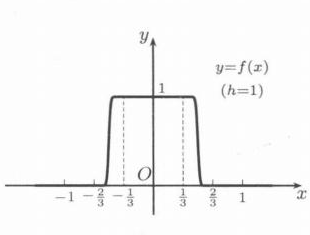
\includegraphics[width=.42\linewidth]{figures/lower/ch14/fig-14-3.png}

  图 14.3
\end{center}

由此出发作积分，就可以归纳地证明：
\[
  \abs{f_n^{(k)}(x)}<\frac{\abs{x}^{n-1-k}}{(n-1-k)!},
\]
其中 $0\leqslant k<n$。

现在对于每个非负整数 $n$ 取 $h=a_nn!$，用上面的方法构造出在 $(-\infty,+\infty)$ 上无限次可微的函数列 $\{u_n(x)\}$，使满足条件
\[
  u_n^{(k)}(0)=0,\ \forall k\ne n,\qquad u_n^{(n)}(0)=a_nn!,
\]
同时有估计 $\displaystyle\abs{u_n^{(k)}(x)}<\frac{\abs{x}^{n-1-k}}{(n-1-k)!},\ \forall0\leqslant k<n$。

现在定义下列函数项级数及其和函数：
\begin{equation}
  u_0(x)+u_1(x)+\cdots+u_n(x)+\cdots=U(x).
  \tag{14.20}
  \label{eq:14.20}
\end{equation}
由以上估计可知，不仅级数 (14.20) 在任意有界闭区间上一致收敛，而且在任意次逐项求导后的级数也一致收敛。因此 $U(x)$ 无穷次可微，且其导数可以用级数的逐项求导来得到。这样就得到 $U^{(n)}(0)=u_n^{(n)}(0)=n!a_n$。
\end{xproof}

\begin{xremark}
根据上述命题，只要取 $\{a_n\}$，使得幂级数 $\displaystyle\sum_{n=0}^{\infty}a_nx^n$ 的收敛半径为 $0$，这样就得到收敛半径为 $0$ 的 Taylor 级数。
\end{xremark}

就问题 2 来说，上册 169 页的例题 6.2.4 已提供了这样的例子。这就是
\[
  f(x)=
  \begin{cases}
    \ee^{-1/x^2},& x\ne0,\\
    0,& x=0.
  \end{cases}
\]
它处处无限次可微，在 $x=0$ 处的任意阶导数值为 $0$，因此在该点的 Taylor 级数的每一项为 $0$，收敛半径当然是 $R=+\infty$。但是这个级数在 $x\ne0$ 的每一点上的和函数值都不等于 $f(x)$ 的值。因此，这个函数在 $x=0$ 处（附近）不能展开为幂级数（参见上册 169 页的图 6.4）。\footnote{将这个函数及其倍数加到任意一个 Maclaurin 级数上去，就可以知道有无限多个函数具有相同的 Maclaurin 级数，但其中至多只有一个函数以此级数为其幂级数展开式。}

解决函数是否能展开为幂级数的工具是第七章中的 Taylor 公式：设 $f$ 在点 $x_0$ 的某个邻域 $U(x_0)$ 中无限次可微，则对于每个 $n$ 有
\[
  f(x)=\sum_{k=0}^{n}\frac{f^{(k)}(x_0)}{k!}(x-x_0)^k+r_n(x),
\]
其中余项可以有多种形式（见命题 7.2.2--7.2.4 或命题 11.4.3）。将此式改写为
\begin{equation}
  r_n(x)=f(x)-\sum_{k=0}^{n}\frac{f^{(k)}(x_0)}{k!}(x-x_0)^k,
  \tag{14.21}
  \label{eq:14.21}
\end{equation}
并与 (14.17) 作比较，就可以看出，这里的 $r_n(x)$ 就是 $f(x)$ 与其 Taylor 级数的第 $n+1$ 个部分和函数之差。因此就可以建立下列基本结论：

\begin{xproposition}[14.4.3]
$f$ 在点 $x_0$ 的邻域 $U(x_0)$ 能展开为幂级数 $\displaystyle\sum_{n=0}^{\infty}a_n(x-x_0)^n$ 的充分必要条件是 $f$ 的 Taylor 公式的余项 (14.21) 在邻域 $U(x_0)$ 内处处收敛于 $0$。
\end{xproposition}
\begin{xproof}
先证必要性。设 $f$ 在点 $x_0$ 的某个邻域 $U(x_0)$ 上是幂级数 $\displaystyle\sum_{n=0}^{\infty}a_n(x-x_0)^n$ 的和函数。根据命题 14.4.1 可知，这个幂级数只能是 Taylor 级数 (14.17)。由于该级数收敛，因此该级数作为收敛级数的余项就是 Taylor 公式的余项 (14.21)。于是已经证明了 $r_n(x)$ 在该邻域内处处收敛于 $0$。

再证充分性。若 $\{r_n(x)\}$ 在某个邻域 $U(x_0)$ 内处处趋于 $0$，则从 (14.21) 可见 Taylor 级数 (14.17) 有正收敛半径，且至少在 $U(x_0)$ 上以 $f(x)$ 为其和函数。
\end{xproof}

\begin{xremark}
由此可见，利用 Taylor 公式的余项在理论上可以同时解决 Taylor 级数 (14.17) 是否有正收敛半径以及其和函数是否等于 $f(x)$ 的问题。
\end{xremark}

\begin{xremark}
初学者往往容易将第七章的 Taylor 公式与本节的 Taylor 级数混淆，因此这里简要地指出两者的差别如下。第七章的 Taylor 公式并不涉及无限项求和问题，其中只有有限项。同时，对于函数 $f$ 的要求也只需要有若干次可微性。这些都与本节的 Taylor 级数不同。在上册 204 页开始引入的 Taylor 公式的余项概念与无穷级数中的余项概念完全不同。在命题 14.4.3 的证明中的关键之处就在于这两个余项在命题的条件下可以等同起来。
\end{xremark}

\subsection{将函数展开为幂级数的基本方法}

与 7.2.2 小节中计算 Taylor 公式的方法类似，将给定的一个函数在指定点附近展开为幂级数有直接法与间接法两种方法。本节中将较多地介绍间接法。这里的原因是容易理解的。所谓\textbf{直接法}或\textbf{直接展开法}，就是利用命题 14.4.1 写出级数 (14.17)，然后再用命题 14.4.3 证明余项趋于 $0$。因此用直接法首先需要计算函数在展开点的所有高阶导数，又为了研究余项，还需要计算 $f$ 的所有高阶导函数，而这往往是更困难的工作。在教科书中也只是对于少数几个初等函数采用直接法得到它们的幂级数展开式。因此我们将较多地介绍间接法。

下面六个基本的 Taylor 级数就是应用间接法的基础，希望初学者把它们作为数学分析中最重要的公式牢牢记住。

1. $\displaystyle\frac1{1-x}=1+x+x^2+\cdots+x^n+\cdots,\ x\in(-1,1)$；

2. $\displaystyle\ee^x=1+x+\frac{x^2}{2!}+\cdots+\frac{x^n}{n!}+\cdots,\ x\in(-\infty,+\infty)$；

3. $\displaystyle\sin x=x-\frac{x^3}{3!}+\frac{x^5}{5!}-\cdots+(-1)^n\frac{x^{2n+1}}{(2n+1)!}+\cdots,\ x\in(-\infty,+\infty)$；

4. $\displaystyle\cos x=1-\frac{x^2}{2!}+\frac{x^4}{4!}-\cdots+(-1)^n\frac{x^{2n}}{(2n)!}+\cdots,\ x\in(-\infty,+\infty)$；

5. $\displaystyle\ln(1+x)=x-\frac{x^2}{2}+\cdots+\frac{(-1)^{n-1}x^n}{n}+\cdots,\ x\in(-1,1]$；

6. $\displaystyle(1+x)^\alpha=1+\alpha x+\frac{\alpha(\alpha-1)}{2!}x^2+\cdots+\frac{\alpha(\alpha-1)\cdots(\alpha-n+1)}{n!}x^n+\cdots$，其中 $\alpha$ 为不等于非负整数的任何实数，而展开式成立的范围当 $\alpha\leqslant-1$ 时为 $(-1,1)$，当 $-1<\alpha<0$ 时为 $(-1,1]$，当 $\alpha>0$ 时为 $[-1,1]$。

\begin{xremark}
上面的 Taylor 级数 6，即二项式级数，是一个十分有用的幂级数展开式。例如上面的级数展开式 1 实际上是二项式级数的特例，只要在其中将 $x$ 换为 $-x$ 并且取 $\alpha=-1$ 即可。只是由于该展开式的重要性，我们单独把它作为一个展开式列出。级数展开式 5 也可以用先对 $\ln(1+x)$ 求导，再对 $\alpha=-1$ 时的二项式级数逐项积分得到。在下面的例题中，我们还会再用二项式级数推出一些常见的初等函数的幂级数展开式。

这里需要说明，所谓间接法并没有明确的范围，实际上只要不是用直接法就都是间接法。\textbf{间接法的理论基础}是幂级数展开的惟一性定理（即命题 14.4.1）。根据这个定理，不论用什么方法，只要所得的幂级数有正收敛半径就可以。其中当然可以使用四则运算和微积分运算。对于乘法运算，由于幂级数在收敛域内部的绝对收敛性，而乘积级数按照幂级数形式写出时恰好就是 Cauchy 乘积，因此在 13.3.2 小节中的命题 13.3.5 已经解决了幂级数的相乘问题。但是对于除法，则需要有新的理论根据。下面是这方面的一个命题，其中的证明取自 [60]。
\end{xremark}

\begin{xproposition}[14.4.4]
设函数 $f$ 在点 $x=0$ 邻近可以展开为幂级数 $1+a_1x+a_2x^2+\cdots+a_nx^n+\cdots$，则其倒函数 $\dfrac1f$ 也可以在点 $x=0$ 邻近展开为幂级数。
\end{xproposition}
\begin{xproof}
从给出收敛半径的 Cauchy-Hadamard 公式可以知道，存在 $r>0$，使得 $\abs{a_n}<r^n$ 对每个 $n=1,2,\ldots$ 成立。（此点请读者根据公式 (14.14) 作出证明。）现在先作形式计算，即求待定的数列 $\{b_n\}$，使得成立
\begin{equation}
  (1+a_1x+a_2x^2+\cdots)(1+b_1x+b_2x^2+\cdots)=1.
  \tag{14.22}
  \label{eq:14.22}
\end{equation}
将左边的乘积展开，并等置两边同次数的乘幂项，就得到计算 $\{b_n\}$ 的递归公式：
\[
  b_1=-a_1,\quad b_2=-a_1b_1-a_2,\quad\ldots,
\]
\[
  b_n=-a_1b_{n-1}-a_2b_{n-2}-\cdots-a_n,\quad\ldots.
\]

现在我们用数学归纳法来证明，对于 $\{b_n\}$ 有下列估计式：
\begin{equation}
  \abs{b_n}<2^{n-1}r^n,\quad n=1,2,\ldots.
  \tag{14.23}
  \label{eq:14.23}
\end{equation}
对于 $n=1$，有 $\abs{b_1}=\abs{a_1}<r$，因此符合 (14.23)。设估计式 (14.23) 对于 $n=1,2,\ldots,k-1$ 成立，则对于 $n=k$ 就有
\[
\begin{aligned}
  \abs{b_k}&\leqslant\abs{a_1b_{k-1}}+\abs{a_2b_{k-2}}+\cdots+\abs{a_{k-1}b_1}+\abs{a_k}\\
  &\leqslant(2^{k-2}+2^{k-3}+\cdots+1+1)r^k=2^{k-1}r^k.
\end{aligned}
\]
因此估计式 (14.23) 成立。

利用这个估计式，从 Cauchy-Hadamard 公式 (14.14) 就知道，幂级数
\[
  1+b_1x+b_2x^2+\cdots+b_nx^n+\cdots
\]
至少在 $\abs{x}<\dfrac1{2r}$ 时收敛。从而当 $\abs{x}<\min\{r,\dfrac1{2r}\}$ 时，等式 (14.22) 不只是作形式运算（即待定系数法）的出发点，而且是严格成立的。这也就是所要的结果：在 $x=0$ 的一个邻域上有幂级数展开式
\[
  \frac1{1+a_1x+\cdots+a_nx^n+\cdots}=1+b_1x+b_2x^2+\cdots+b_nx^n+\cdots.
\]
\end{xproof}

\begin{xremark}
在这个命题的基础上再结合级数相乘，就可以得到幂级数相除的一般结论：若 $f=g/h$，其中函数 $g$ 和 $h$ 在点 $x_0$ 的邻近都可以展开为幂级数，且 $h(x_0)\ne0$，则 $f$ 也可以在点 $x_0$ 邻近展开成幂级数，同时这个级数的系数可以用类似于上述命题证明中的待定系数法来得到。
\end{xremark}

\begin{xremark}
在 [18] 第二卷 446 小节中证明了更为一般的命题。这里只叙述其结论，证明从略。还可以参考 [15] 的第二章。
\end{xremark}

\begin{xproposition}
设幂级数展开式 $y=f(x)=\displaystyle\sum_{n=0}^{\infty}a_nx^n$ 在点 $x=0$ 邻近成立，又有幂级数展开式 $z=\varphi(y)=\displaystyle\sum_{n=0}^{\infty}b_ny^n$ 在区间 $(-\rho,\rho)$ 中成立，如果满足条件 $\abs{a_0}=\abs{f(0)}<\rho$，则复合函数 $z=\varphi(f(x))$ 在点 $x=0$ 的邻近可以展开为幂级数，同时其系数可以用级数代入级数的待定系数法得到。
\end{xproposition}

\subsection{例题}

这一节的内容与上册 7.2.2 和 7.2.3 小节的部分内容有密切联系。那里的许多 Taylor 公式的计算可以作为本节的特例得到，而且当时的间接法还只有级数代入级数之类的方法，现在则还可以用逐项求和与逐项求导方法。

以下第一个例题中的两个初等函数的 Maclaurin 展开式可以用直接法得到，也可以用逐项积分的间接法得到，后者无疑更为方便。初学者应当重视这些基本训练，同时也应当记住这两个基本的 Taylor 级数展开式。

\begin{xexample}[14.4.1]
用间接法求 $\arctan x$ 与 $\arcsin x$ 的 Maclaurin 级数展开式。
\end{xexample}
\begin{xsolution}
(1) 由于
\[
  (\arctan x)'=\frac1{1+x^2}=\sum_{n=0}^{\infty}(-1)^nx^{2n},\quad x\in(-1,1),
\]
用逐项积分就得到
\[
  \arctan x=x-\frac{x^3}{3}+\cdots+\frac{(-1)^nx^{2n+1}}{2n+1}+\cdots,\quad x\in(-1,1).
\]

(2) 由于
\[
  (\arcsin x)'=\frac1{\sqrt{1-x^2}}=1+\sum_{n=1}^{\infty}\frac{(2n-1)!!}{(2n)!!}x^{2n},\quad x\in(-1,1),
\]
用逐项积分就得到
\[
  \arcsin x=x+\frac{x^3}{6}+\cdots+\frac{(2n-1)!!}{(2n)!!(2n+1)}x^{2n+1}+\cdots,\quad x\in(-1,1).
\]
注意：用 Abel 第二定理知道两个展开式都在端点 $x=\pm1$ 处成立。
\end{xsolution}

\begin{xexample}[14.4.2]
现在求正弦和余弦之外的四个基本三角函数的 Maclaurin 展开式（其中 $\cot x$ 和 $\csc x$ 是在乘以因子 $x$ 之后的 Maclaurin 展开式）。仿照上册 216 页中的做法，并应用命题 14.4.4，就得到 Maclaurin 级数展开式
\begin{equation}
  \frac{x}{\ee^x-1}=B_0+\frac{B_1}{1!}x+\frac{B_2}{2!}x^2+\cdots+\frac{B_n}{n!}x^n+\cdots,
  \tag{14.24}
  \label{eq:14.24}
\end{equation}
其中左边的表达式在点 $x=0$ 处用其极限值 $1$ 来代替。与 7.2.3 小节中的记号相同，$\{B_n\}$ 为 Bernoulli 数，其中 $B_1=-1/2$，当 $n$ 为大于 $1$ 的奇数时 $B_n=0$。以下采用记号 $\overline B_n=(-1)^{n-1}B_{2n}\ (n\geqslant1)$。

由此出发就可以与例题 7.2.8 和 7.2.9 类似地得到 Maclaurin 级数展开式
\begin{equation}
  x\cot x=1-\frac{\overline B_1 2^2}{2!}x^2-\frac{\overline B_2 2^4}{4!}x^4-\cdots-\frac{\overline B_n 2^{2n}}{(2n)!}x^{2n}+\cdots,
  \tag{14.25}
  \label{eq:14.25}
\end{equation}
\begin{equation}
  \tan x=\frac{\overline B_1(2^2-1)2^2}{2!}x+\frac{\overline B_2(2^4-1)2^4}{4!}x^3+\cdots+\frac{\overline B_n(2^{2n}-1)2^{2n}}{(2n)!}x^{2n-1}+\cdots,
  \tag{14.26}
  \label{eq:14.26}
\end{equation}
再利用三角恒等式 $\displaystyle\csc x=\frac12\left(\cot\frac x2+\tan\frac x2\right)$，即可得到
\begin{equation}
  x\csc x=1+\sum_{n=1}^{\infty}\frac{\overline B_n(2^{2n}-2)}{(2n)!}x^{2n}.
  \tag{14.27}
  \label{eq:14.27}
\end{equation}
最后，回顾例题 7.2.7 并应用命题 14.4.4 就可以得到
\begin{equation}
  \sec x=E_0-\frac{E_2}{2!}x^2+\cdots+\frac{(-1)^nE_{2n}}{(2n)!}x^{2n}+\cdots,
  \tag{14.28}
  \label{eq:14.28}
\end{equation}
其中 $\{E_{2n}\}$ 为 Euler 数（见上册 215 页）。\footnote{根据第十六章例题 16.2.3 后的注，利用渐近等式 (16.13)，即 $\overline B_n\sim\dfrac{2(2n)!}{(2\pi)^{2n}}$，就很容易确定 (14.24)、(14.25)、(14.26) 和 (14.27) 这四个 Maclaurin 级数的收敛半径分别为 $2\pi,\pi,\pi/2$ 和 $\pi$。又从 $\sec x=(\tan x/x)\cdot(x\csc x)$ 和级数乘积定理，就可以推出 (14.28) 的收敛半径为 $\pi/2$。最后，根据 Abel 第二定理可确定所有这些展开式的准确的成立范围。}
\end{xexample}

\begin{xexample}[14.4.3]
求 $f(x)=\dfrac1{1+x+x^2}$ 在 (1) 点 $x_0=0$ 和 (2) 点 $x_0=-\dfrac12$ 处的幂级数展开式。
\end{xexample}
\begin{xsolution}
(1) 这时可以如下计算：
\[
\begin{aligned}
  f(x)&=\frac1{1+x+x^2}=\frac{1-x}{1-x^3}=(1-x)\sum_{n=0}^{\infty}x^{3n}\\
  &=\sum_{n=0}^{\infty}x^{3n}-\sum_{n=0}^{\infty}x^{3n+1}\\
  &=(1+x^3+x^6+\cdots+x^{3n}+\cdots)-(x+x^4+x^7+\cdots+x^{3n+1}+\cdots)\\
  &=1-x+x^3-x^4+\cdots+x^{3n}-x^{3n+1}+\cdots,\quad x\in(-1,1).
\end{aligned}
\]
这就是所求的幂级数展开式。

(2) 为了将函数 $f$ 展开成关于 $x+\dfrac12$ 的乘幂的幂级数，可计算如下：
\[
\begin{aligned}
  f(x)&=\frac1{1+x+x^2}=\frac1{\dfrac34+\left(x+\dfrac12\right)^2}=\frac43\cdot\frac1{1+\dfrac43\left(x+\dfrac12\right)^2}\\
  &=\frac43\sum_{n=0}^{\infty}(-1)^n\left[\frac43\left(x+\frac12\right)^2\right]^n
  =\frac43\sum_{n=0}^{\infty}\left(-\frac43\right)^n\left(x+\frac12\right)^{2n}.
\end{aligned}
\]
其中应用了上一节中列举的基本公式之 1，即 $\dfrac1{1-x}$ 的幂级数展开式。从以上计算过程不难看出级数展开式成立的范围为
\[
  \abs{\frac2{\sqrt3}\left(x+\frac12\right)}<1,
\]
即 $\displaystyle x\in\left(-\frac12-\frac{\sqrt3}{2},-\frac12+\frac{\sqrt3}{2}\right)$。
\end{xsolution}

\begin{xremark}
如果注意到
\[
  \sin\frac{2(n+1)\pi}{3}=
  \begin{cases}
    \dfrac{\sqrt3}{2},&n=3k,\\[3pt]
    -\dfrac{\sqrt3}{2},&n=3k+1,\quad k=0,1,2,\ldots,\\[3pt]
    0,&n=3k+2,
  \end{cases}
\]
就可以将 (1) 的幂级数展开式改写为
\[
  f(x)=\frac2{\sqrt3}\sum_{n=0}^{\infty}\sin\frac{2(n+1)\pi}{3}x^n,\quad x\in(-1,1).
\]
\end{xremark}

\begin{xexample}[14.4.4]
求函数 $f(x)=\ln^2(1+x)$ 的 Maclaurin 级数展开式。
\end{xexample}
\begin{xsolution}
用级数乘法即可得到在 $(-1,1)$ 中成立幂级数展开式：
\begin{equation}
  \ln^2(1+x)=2\sum_{n=2}^{\infty}\frac{(-1)^n}{n}\left(1+\frac12+\frac13+\cdots+\frac1{n-1}\right)x^n.
  \tag{14.29}
  \label{eq:14.29}
\end{equation}
当 $x=1$ 时右边级数收敛，从 Abel 第二定理知该展开式在 $x=1$ 时仍成立。
\end{xsolution}

\begin{xexample}[14.4.5]
设 $a$ 不是 $\pi$ 的整倍数，求函数 $\displaystyle\frac{x\sin a}{1-2x\cos a+x^2}$ 的 Maclaurin 级数展开式。
\end{xexample}
\begin{xsolution}
用待定系数法计算如下。设
\[
  \frac{x\sin a}{1-2x\cos a+x^2}=\sum_{n=0}^{\infty}a_nx^n,
\]
两边乘以 $1-2x\cos a+x^2$ 并等置两边同次项，就可求出
\[
  a_0=0,\quad a_1=\sin a,\quad a_2=\sin2a,\quad\ldots,\quad a_n=\sin na,\quad\ldots.
\]
因此
\[
  \frac{x\sin a}{1-2x\cos a+x^2}=\sum_{n=1}^{\infty}x^n\sin na.
\]
容易看出右边的级数在 $x\in(-1,1)$ 上收敛。而当 $a$ 不是 $\pi$ 的整倍数时，数列 $\{\sin na\}$ 不趋于 $0$，因此级数的收敛域就是 $(-1,1)$。
\end{xsolution}

上面所举的例题都用间接展开法，但这并不等于说，间接法总是比直接法好。下面这道例题，用直接法要比用间接法容易一些。

\begin{xexample}[14.4.6]
求 $f(x)=\ee^x\sin x$ 的 Maclaurin 级数展开式。
\end{xexample}
\begin{xsolution}
如果用间接展开法，则需要将 $\ee^x$ 与 $\sin x$ 的 Maclaurin 级数展开式相乘，运算将较为复杂。因此我们采用直接展开法。首先，可用数学归纳法证明公式
\[
  f^{(n)}(x)=(\sqrt2)^n\ee^x\sin\left(x+\frac{n\pi}{4}\right),
\]
由此得到
\[
  f^{(n)}(0)=(\sqrt2)^n\sin\frac{n\pi}{4},\quad n=1,2,3,\ldots.
\]
这样就得到所求的 Maclaurin 级数为
\begin{equation}
  \sum_{n=0}^{\infty}\frac{(\sqrt2)^n\sin\dfrac{n\pi}{4}}{n!}x^n.
  \tag{14.30}
  \label{eq:14.30}
\end{equation}
按照直接法的一般步骤，到这里为止还不知道级数 (14.30) 是否收敛于 $\ee^x\sin x$，因此需要应用命题 14.4.3 去研究 Taylor 公式的余项。但是这里可以避免这一步。利用 $\ee^x$ 和 $\sin x$ 的 Maclaurin 级数展开式均在 $(-\infty,+\infty)$ 成立，因此处处绝对收敛。应用级数乘积定理（命题 13.3.5），就可以知道 $\ee^x\sin x$ 也能够展开为幂级数，且收敛半径也是 $+\infty$。再利用幂级数展开的惟一性定理（即命题 14.4.1），可见 (14.30) 必定在 $(-\infty,+\infty)$ 上收敛于 $\ee^x\sin x$。
\end{xsolution}

\subsection{练习题}

\begin{xexercise}
\begin{enumerate}
  \item 将函数 $f(x)=\dfrac1{a-x}\ (a\ne0)$ 分别按 $x$、$x-b$、$\dfrac1x$ 的乘幂展开。
  \item 将函数 $f(x)=\ln x$ 展开为 $\dfrac{x-1}{x+1}$ 的幂级数。
  \item 设函数 $f$ 在区间 $(-a,a)\ (a>0)$ 上无限次可微，且导函数序列 $\{f^{(n)}\}$ 在 $(-a,a)$ 上一致有界，证明：$f$ 在 $(-a,a)$ 上可以展开为 Maclaurin 级数。
  \item 设函数 $f$ 在 $(-\infty,+\infty)$ 上无穷次可导，并且其导函数列在 $(-\infty,+\infty)$ 上一致有界。如果存在正数数列 $\{x_n\}$，使 $\displaystyle\lim_{n\to\infty}x_n=0$ 且 $f(x_n)=0,\ n=1,2,\ldots$。证明：$f(x)=0$。
  \item 求下列函数的 Maclaurin 展开式，并确定其成立范围：
  \begin{enumerate}[label=(\arabic*)]
    \item $\sqrt{4-x}$；
    \item $a^x,\ a>0$；
    \item $\ln(1+3x+2x^2)$；
    \item $\arctan\dfrac{2x}{1-x^2}$；
    \item $\dfrac1{1+x+x^2+x^3+x^4}$；
    \item $\dfrac{\ee^{x^2}}{1-x^2}$；
    \item $\displaystyle\frac{\dd}{\dd x}\left(\frac{\ee^x-1}{x}\right)$；
    \item $\displaystyle\int_0^x\frac{1-\cos t}{t^2}\,\dd t$。
  \end{enumerate}
  \item 将下列函数在指定点展开为幂级数：
  \begin{enumerate}[label=(\arabic*)]
    \item $\dfrac1{3+x},\ x=2$；
    \item $\ln\dfrac1{3+2x+x^2},\ x=-1$；
    \item $\ln x,\ x=3$；
    \item $\dfrac{x-1}{x+1},\ x=1$；
    \item $\sin x,\ x=\dfrac\pi6$。
  \end{enumerate}
\end{enumerate}
\end{xexercise}

\section{对于教学的建议}

\subsection{学习要点}

1. 一致收敛性是函数项级数与函数列中最重要也是最困难的概念。对于这个概念的掌握需要花很大力气。初学者首先要能正确叙述“一致性”的有关论述，记住一些重要的反例，如函数列 $\{x^n\}$ 在 $[0,1]$ 上的一致收敛性讨论可以很形象地体现出“一致性”论述中的要点。其次，要能体会一致收敛性在将通项函数或函数列的分析性质“传递”给和函数或极限函数时的重要性。

2. 本章的一个难点是在函数项级数与函数列的概念中，同时出现了两个变量：正整数变量 $n$ 与连续变量 $x$。在处理收敛、一致收敛问题或讨论和函数与极限函数的分析性质时，学生往往不容易分辨清楚何时该将哪个变量看成常量。可以向学生强调的是，在考虑两个极限的累次极限时，计算第一个极限时，应该把另一个变量看作常量；同样，对极限
\[
  \lim_{n\to\infty}\sup\{\abs{S_n(x)-S(x)}\mid x\in E\},
\]
计算 $\sup\{\abs{S_n(x)-S(x)}\mid x\in E\}$ 时，要把 $n$ 看作常数。另外，在讨论与点收敛有关的问题时，$x$ 可以看作常数，而讨论与一致收敛有关的问题时，则 $x$ 一般不能看作常数。

3. 尽管一致收敛性有很多判别法，但最常用的一致收敛性判别法还是 M-判别法，能用多种手段找出优级数是一致收敛性判别法部分的基本教学要求。

4. 函数项级数的和函数的连续性、逐项求导、逐项积分等内容本质上是运算次序的交换。这里极限顺序交换的基本原理是很基本的一个事实，在一系列问题中起指导作用。

5. 和函数（极限函数）在一个区间上的局部分析性质，如连续性、可微性等都可以通过在每一点的邻域上的讨论而得。因此，可以用内闭一致收敛取代一致收敛，即使是求积分，也可先考虑内闭区间上的逐项积分。如证明 Riemann 的 zeta-函数 $\displaystyle\zeta(x)=\sum_{n=1}^{\infty}\frac1{n^x}$ 在 $(1,+\infty)$ 上的无穷次可微，求积分
\[
  \int_0^1\left(\sum_{n=1}^{\infty}x^n\ln x\right)\dd x
\]
的值等都是一些典型的例子。

6. 一般项的函数项级数的讨论可围绕一些重要的例子，如 $\displaystyle\sum_{n=1}^{\infty}\frac{\sin nx}{n^p}$ 等展开，抓住重点，举一反三。

7. 幂级数部分的教学除了以 Abel 定理为中心的基本理论之外，应注意应用能力的培养，如间接展开、定积分计算、求重要级数的和等。

8. 幂级数是一种特殊的函数项级数，因此，本章前两节中关于函数项级数的一切结论，对于幂级数都是适用的。在教学中，遇到需要用这些结论时，可复习一下一般函数项级数的对应结论，以起到温故知新的作用。

\subsection{参考题}

\paragraph{第一组参考题}

\begin{xreferenceproblem}
\begin{enumerate}
  \item 试举例：在 $[0,1]$ 上一致收敛于连续函数的函数列 $\{S_n(x)\}$，但每个 $S_n(x)$ 在 $[0,1]$ 上处处不连续。
  \item 用逐项求导方法写出函数 $\displaystyle\zeta(x)=\sum_{n=1}^{\infty}\frac1{n^x}$ 在 $(1,+\infty)$ 上的任意阶导数的表达式，并证明运算的合理性。
  \item 证明 Dirichlet 级数 $\displaystyle\sum_{n=1}^{\infty}\frac{a_n}{n^x}$ 的收敛域具有以下特性：若存在 $x_1,x_2$，使 $x=x_1$ 时级数发散，而当 $x=x_2$ 时级数收敛，则一定存在 $r\in(-\infty,+\infty)$，使 $x<r$ 时级数发散，而 $x>r$ 时级数收敛。
  \item 设 $f\in C[0,1]$，定义函数列 $S_n(x)=x^nf(x),\ x\in[0,1],\ n=1,2,\ldots$，证明：$\{S_n(x)\}$ 在 $[0,1]$ 上一致收敛的充分必要条件是 $f(1)=0$。
  \item 设数列 $\{r_n\}$ 是 $[0,1]$ 区间内的所有有理点的一个排列，证明函数
  \[
    f(x)=\sum_{n=1}^{\infty}\frac{\abs{x-r_n}}{3^n},\quad x\in[0,1]
  \]
  具有性质：(1) 处处连续；(2) 在 $[0,1]$ 的每个无理点处可微，而在每个有理点处不可微。
  \item 设函数 $f$ 在区间 $[0,1]$ 上无穷次可微且不恒等于 $0$，$f^{(n)}(0)=0,\ n=0,1,\ldots$。如果函数列 $\{a_nf^{(n)}\}$ 在区间 $[0,1]$ 上一致收敛于 $0$，其中 $\{a_n\}$ 为一给定的数列，证明：$\displaystyle\lim_{n\to\infty}n!a_n=0$。
  \item 用幂级数方法证明级数乘积的一个基本结果（即命题 13.3.7）：设 $\displaystyle\sum_{n=1}^{\infty}a_n$、$\displaystyle\sum_{n=1}^{\infty}b_n$ 和它们的 Cauchy 乘积 $\displaystyle\sum_{n=1}^{\infty}c_n$ 均收敛，且分别以 $A,B,C$ 为和，则 $C=AB$。
  \item 求下列函数的 Maclaurin 展开式：
  \begin{enumerate}[label=(\arabic*)]
    \item $\dfrac{\arcsin x}{\sqrt{1-x^2}}$；
    \item $\dfrac{\ln(x+\sqrt{1+x^2})}{\sqrt{1+x^2}}$；
    \item $\left(\dfrac{\arcsin x}{x}\right)^2$（函数在点 $x=0$ 处用极限值定义）。
  \end{enumerate}
  \item 设数列 $\{a_n\}$ 有极限 $L$，证明：$\displaystyle f(x)=\sum_{n=1}^{\infty}a_nx^n$ 在 $(-1,1)$ 上有定义，且 $\displaystyle\lim_{x\to1-}(1-x)f(x)=L$。
  \item 设多项式序列 $\{P_n\}$ 在 $(-\infty,+\infty)$ 上一致收敛于 $P$，证明：$P$ 也是多项式。
  \item 设 $\{P_n\}$ 是次数不超过 $D$ 的多项式序列，证明：若该序列于区间 $[0,1]$ 上收敛，则也一定一致收敛。
  \item 设 $\displaystyle\sum_{n=0}^{\infty}a_nx^n$ 为 $f$ 在 $(-\infty,+\infty)$ 上的 Maclaurin 级数展开式，证明：$\displaystyle\sum_{n=0}^{\infty}a_nx^n$ 在 $(-\infty,+\infty)$ 上一致收敛的充分必要条件是 $f$ 为多项式。
  \item 设 $C(a)$ 为 $(1+x)^a$ 的 Maclaurin 级数展开式中 $x^{2003}$ 项的系数，计算积分
  \[
    \int_0^1 C(-y-1)\left(\frac1{y+1}+\frac1{y+2}+\frac1{y+3}+\cdots+\frac1{y+2003}\right)\dd y.
  \]
  \item 求级数和 $\displaystyle\sum_{m=1}^{\infty}\sum_{n=1}^{\infty}\frac{m^2n}{3^m(n3^m+m3^n)}$。
  \item 甲乙两人掷骰子，两人依次轮流掷并且由甲掷第一次，问第一个六点由甲掷出的概率是多少？
  \item 某侨商捐资给母校设立奖学基金。该基金存入银行，每年可以得到 $a\%$ 的利息。奖学金按如下数目发放：基金存入银行当日发放一万元，第二年同一天发放二万元，以后每年同一日发放，发放金额比前一年多一万元。要使这笔奖学金能够永远按此规律发放下去，该侨商至少应捐资多少元？
\end{enumerate}
\end{xreferenceproblem}

\paragraph{第二组参考题}

\begin{xreferenceproblem}
\begin{enumerate}
  \item 设 $\{f_n\}$ 是在 $[a,b]$ 上的可积函数列，且于 $[a,b]$ 上一致有界，若已知 $\{f_n\}$ 在 $[a,b]$ 上收敛，证明：积分值所成的数列必有极限 $\displaystyle\lim_{n\to\infty}\int_a^b f_n$。
  \item 若在 $[a,b]$ 上的可积函数列 $\{f_n\}$ 一致收敛于极限函数 $f$，证明：$f\in R[a,b]$，且有
  \[
    \lim_{n\to\infty}\int_a^b f_n(x)\,\dd x=\int_a^b f(x)\,\dd x.
  \]
  \item 设具有相同单调性的单调函数列 $\{f_n\}$ 在区间 $[a,b]$ 上收敛于 $f\in C[a,b]$，则 $\{f_n\}$ 在 $[a,b]$ 上一致收敛。
  \item 设 $\{f_n\}$ 是 $[a,b]$ 上的连续函数列，并已知对于每个 $x\in[a,b]$，数列 $\{f_n(x)\}$ 单调增加收敛于 $f(x)$，证明：$f$ 在 $[a,b]$ 上必有最小值。又问：若将最小值换为最大值，或将 $[a,b]$ 换为 $(a,b)$，则结论如何？
  \item 设 $\{f_n\}$ 为 $[a,b]$ 上的连续可微函数列，且存在 $\{x_n\}\subset[a,b]$，使 $f_n(x_n)=x_n,\ n=1,2,\ldots$。如果导函数列 $\{f_n'\}$ 在 $[a,b]$ 上一致收敛，证明：
  \begin{enumerate}[label=(\arabic*)]
    \item 函数列 $\{f_n\}$ 有子列 $\{f_{n_k}\}$ 在 $[a,b]$ 上一致收敛；
    \item 设 $\{f_{n_k}\}$ 的极限函数为 $f$，则存在 $x_0\in[a,b]$，使 $f(x_0)=x_0$；
    \item $f$ 在 $[a,b]$ 上连续可微，且在 $[a,b]$ 上 $f'(x)=\displaystyle\lim_{n\to\infty}f_n'(x)$。
  \end{enumerate}
  \item 设在区间 $[a,b]$ 上的连续函数项级数 $\displaystyle\sum_{n=1}^{\infty}u_n(x)$、$\displaystyle\sum_{n=1}^{\infty}v_n(x)$ 的通项之间满足条件
  \[
    \abs{u_n(x)}\leqslant v_n(x),\quad n=1,2,\ldots,
  \]
  又设 $\displaystyle\sum_{n=1}^{\infty}v_n(x)$ 的和函数在 $[a,b]$ 上连续，证明：$\displaystyle\sum_{n=1}^{\infty}u_n(x)$ 的和函数也在 $[a,b]$ 上连续。
  \item 证明：对任意 $n$ 和 $x$ 成立不等式
  \[
    \abs{\sum_{k=1}^{n}\frac{\sin kx}{k}}\leqslant2\sqrt\pi.
  \]
  \item 利用幂级数展开证明（上册 374 页的题 15）不等式：
  \[
    0<\frac12\ln\frac{1+x}{1-x}-x<\frac{x^3}{3(1-x^2)},\quad 0<x<1.
  \]
  \item 利用幂级数展开证明：对一切 $n\in\NN_+$ 和实数 $x$ 成立不等式：
  \[
    \abs{\ee^x-\left(1+\frac xn\right)^n}
    \leqslant \ee^{\abs{x}}-\left(1+\frac{\abs{x}}n\right)^n
    <\frac{x^2\ee^{\abs{x}}}{2n}.
  \]
  \item 设级数 $\displaystyle\sum_{n=0}^{\infty}a_n$ 的部分和数列为 $S_n=a_0+a_1+\cdots+a_n$，$\sigma_n=(S_0+S_1+\cdots+S_{n-1})/n,\ n=1,2,\ldots$，且有极限 $\displaystyle\lim_{n\to\infty}\sigma_n=S$，即级数 $\displaystyle\sum_{n=0}^{\infty}a_n$ 的 Cesàro 和为 $S$（参见 39 页上第十三章末的几个参考题），证明：
  % SOURCE-ERR: 原书此处印作 n=0,1,\ldots；n=0 时分母为 0，此处改为 n=1,2,\ldots。
  \begin{enumerate}[label=(\arabic*)]
    \item $\displaystyle\sum_{n=0}^{\infty}a_nx^n$ 在 $(-1,1)$ 上收敛；
    \item 在 $(-1,1)$ 上成立
    \[
      \sum_{n=0}^{\infty}a_nx^n=(1-x)^2\sum_{n=0}^{\infty}(n+1)\sigma_{n+1}x^n;
    \]
    \item 记 $S(x)=\displaystyle\sum_{n=0}^{\infty}a_nx^n,\ x\in(-1,1)$，则有 $\displaystyle\lim_{x\to1-}S(x)=S$。
  \end{enumerate}
  \item 设 $\{a_n\}$ 与 $\{b_n\}$ 为正数数列，幂级数 $\displaystyle\sum_{n=0}^{\infty}a_nx^n$ 的收敛半径为 $1$，且在 $x=1$ 处发散。如果 $\displaystyle\lim_{n\to\infty}\frac{b_n}{a_n}=A$，证明：
  \[
    \lim_{x\to1-}\frac{\displaystyle\sum_{n=0}^{\infty}b_nx^n}{\displaystyle\sum_{n=0}^{\infty}a_nx^n}=A.
  \]
  \item 证明：如果正项级数 $\displaystyle\sum_{n=0}^{\infty}c_n=A$，则
  \[
    \lim_{x\to1-}\left(\sum_{n=0}^{\infty}c_nx^n\right)=A.
  \]
  （本题为上题之特例，但也可以用其他方法做。）
  \item 设 $f$ 在区间 $[0,r)$ 上无限次可微，且 $f$ 及其所有导函数都是非负的，证明：$f$ 的 Maclaurin 级数展开式在 $[0,r)$ 上成立：
  \[
    f(x)=\sum_{n=0}^{\infty}\frac{f^{(n)}(0)}{n!}x^n.
  \]
  \item （生成函数法）设 $\{a_n\}$ 为 Fibonacci 数列：$a_0=a_1=1$，$a_n=a_{n-1}+a_{n-2},\ \forall n\geqslant2$，定义
  \[
    f(x)=a_0+a_1x+a_2x^2+\cdots+a_nx^n+\cdots
  \]
  为 $\{a_n\}$ 的\textbf{生成函数}。试求出 $f$，并由此求出 $\{a_n\}$ 的解析表达式，同时求出该数列的\textbf{增长数}：$\displaystyle\lim_{n\to\infty}\frac{a_{n+1}}{a_n}$（参见上册 48 页）。
  \item 利用上题的生成函数方法证明组合学中的 Vandermonde（范德蒙德）恒等式：
  \[
    \sum_{k=0}^{n}{\alpha\choose k}{\beta\choose n-k}={\alpha+\beta\choose n},
  \]
  并由此推出
  \[
    \sum_{k=0}^{n}{n\choose k}^2={2n\choose n}.
  \]
\end{enumerate}
\end{xreferenceproblem}
